\documentclass[conference]{IEEEtran}
 
\bibliographystyle{IEEEtran}
\usepackage{amsmath,amsthm}
\usepackage{listings}
\usepackage{tikz}
\usepackage{subfigure}
\usepackage{multirow}
\usepackage{pgfplots}
\usepackage{booktabs}
\usepackage{dcolumn}
\usepackage{cancel}
\usepackage{graphics}

\newcommand{\infrule}[2]{\displaystyle\frac{\displaystyle\strut{#1}}{\displaystyle\strut {#2}}}
\newcommand{\deref}{\ast}
\newcommand{\rread}[1]{\mbox{\em Read}(#1)}
\newcommand{\rwrite}[1]{\mbox{\em Write}(#1)}
\newcommand{\lca}[2]{#1 \sqcup #2}
\newcommand{\rleq}{\leq}
\newcommand{\interval}[1]{\mbox{\em interval}(#1)}
\newcommand{\context}[1]{\mbox{\em context}(#1)}
\newtheorem{theorem}{Theorem} 
\newtheorem{lemma}[theorem]{Lemma}
\newtheorem{observation}[theorem]{Observation}

\begin{document}

\pdfpagewidth=8.5in
\pdfpageheight=11in

\title{Legion: Expressing Locality and Independence with Logical Regions}
\author{
\IEEEauthorblockN{Michael Bauer\IEEEauthorrefmark{1},
%\authorinfo(Stanford University, email: \mbox{mebauer@cs.stanford.edu}
Sean Treichler\IEEEauthorrefmark{1}, 
%\authorinfo(Stanford University, email: \mbox{sjt@cs.stanford.edu}
Elliott Slaughter\IEEEauthorrefmark{1}, 
% \authorinfo(Stanford University, email: \mbox{slaughter@cs.stanford.edu}
Alex Aiken\IEEEauthorrefmark{1}  
%\authorinfo(Stanford University, email: \mbox{aiken@cs.stanford.edu}
%\email{aiken@cs.stanford.edu}
}
\IEEEauthorblockA{
\IEEEauthorrefmark{1}{Computer Science Department, Stanford University}
}
}

\maketitle


\begin{abstract}
Modern parallel architectures have both heterogeneous processors and
deep, complex memory hierarchies.  We present Legion, a programming
model and runtime system for achieving high performance on these
machines.  Legion is organized around {\em logical regions}, which
express both locality and independence of program data, and {\em
  tasks}, functions that perform computations on regions.  We describe
a runtime system that dynamically extracts parallelism from
Legion programs, using a distributed, parallel scheduling algorithm
that identifies both independent tasks and nested parallelism.  Legion
also enables explicit, programmer controlled movement of data through
the memory hierarchy and placement of tasks based on locality
information via a novel mapping interface.  We evaluate our Legion
implementation on three applications: fluid-flow on a regular grid,
a three-level AMR code solving a heat diffusion equation, and 
a circuit simulation.
%
% FIXME: put some performance numbers here
%
\end{abstract}

\section{Introduction}
\label{sect:intro}
%Put intro text here \cite{Fatahalian06}

Modern parallel machines are increasingly complex, with deep,
distributed memory hierarchies and heterogeneous processing units.  Because the
costs of communication within these architectures vary by several orders of magnitude, 
the penalty for mistakes in the placement of data or computation is usually very poor performance.  Thus,
to achieve good performance the programmer
and the programming system must reason about {\em locality} (data resident
close to computation that uses it) and {\em independence} (computations
operating on disjoint data, and therefore not requiring communication and able to be placed in possibly distant parts of the machine).  
Most contemporary
programming systems have no facilities for the programmer to express locality
and independence.  The few languages that do focus primarily on
array-based locality \cite{Fatahalian06,CHAPEL04,UPC99} and 
avoid irregular pointer data structures.  
%
% FIXME
% Sean would like a bit more on why other systems don't support pointer data structures (e.g., the difficulty of
% alias analysis.  I thought about it and feel it is too much of a digression: mentioning that in the first paragraph
% makes it sound like it will be an important part of the paper.
%
%encode such structures in arrays, which 
%data structures encoded in arrays which are impossible for compilers
%and runtime systems to reason about with regard to locality and independence.

In this paper we describe Legion, a parallel programming system based
on using {\em logical regions} to describe the organization of data
and to make explicit relationships useful for reasoning about locality
and independence.
A logical region names a set of objects.  Logical regions are first-class 
values in Legion and may be dynamically allocated, deleted and stored
in data structures. Regions can also be passed as arguments
to distinguished functions called {\em tasks} that access the data in
those regions, providing locality information.  Logical regions may be
{\em partitioned} into disjoint or aliased (overlapping) {\em subregions}, providing
information for determining independence of computations.
Furthermore, computations access logical regions with particular {\em
  privileges} ({\em read-only}, {\em read-write}, and {\em reduce}) and {\em coherence} (e.g., {\em exclusive access} and {\em
  atomic access}, among others).  Privileges express how a task may use
its region arguments, providing data dependence information that
is used to guide the extraction of parallelism.  For example, if two tasks
access the same region with read-only privileges the two tasks
can potentially be run in parallel.
Coherence properties express the required semantics of concurrent region accesses.
For example, if the program executes $f_1(r); f_2(r)$ and tasks $f_1$
and $f_2$ both require {\em exclusive} access to region $r$, then Legion guarantees the result will
be as if $f_1(r)$ completes before $f_2(r)$ begins.   On the other hand, if
the tasks access $r$ with {\em atomic} coherence, then Legion
guarantees only atomicity of the tasks with respect to $r$: either task $f_1(r)$
appears to run entirely before $f_2(r)$ or vice versa.

Logical regions do not commit to any particular layout of the data or
placement in the machine.  At runtime, each logical region has one or
more {\em physical instances} assigned to specific memories .  It is often useful to have multiple
physical instances of a logical region (e.g., to duplicate read-only data, or to allow
independent reductions that are later combined).

To introduce the programming model, we present
a circuit simulation in
Section~\ref{sec:ex}, illustrating regions, tasks,
permissions and coherence properties, the interactions between them,
and how these building blocks are assembled into a Legion
program.  Subsequent sections each describe a contribution in the
implementation and evaluation of Legion:

\lstset{
  captionpos=b,
  language=C++,
  basicstyle=\scriptsize,
  numbers=left,
  numberstyle=\tiny,
  columns=fullflexible,
  stepnumber=1,
  escapechar=\#,
  keepspaces=true,
  literate={<}{{$\langle$}}1 {>}{{$\rangle$}}1,
  morekeywords={region_relation,region,coloring,partition,spawn},
  deletekeywords=float,
}
\begin{lstlisting}[float={t},label={lst:code_ex},caption={Circuit Simulation Code Example}]
struct Node<rn>    { Node<rn>@rn next;    float charge, capacitance; }
struct Wire<rn,rn2,rw> { Wire<rn,rn2,rw>@rw next;
                                          Node<rn2>@rn in_node, out_node; float current, ... ; }
region_relation Circuit {
  region< Node<r_all_nodes> >                        r_all_nodes;
  region< Wire<r_all_nodes,r_all_nodes,r_all_wires> >       r_all_wires;
  Node<r_all_nodes>@r_all_nodes                   first_node;
  Wire<r_all_nodes,r_all_wires>@r_all_wires   first_wire;
}
region_relation CircuitPiece<rn, rw> {
  region< Node<rn_pvt+rn_shr> >                                 rn_pvt (#$\prec$# rn), rn_shr (#$\prec$# rn);
  region< Node<rn> >                                                   rn_ghost (#$\prec$# rn);
  region< Wire<rn_pvt+rn_shr+rn_ghost,rn,rw_pvt> >  rw_pvt (#$\prec$# rw);
  Node<rn_pvt+rn_shr>@(rn_pvt+rn_shr)                     first_node;
  Wire<rn_pvt+rn_shr+rn_ghost,rn,rw_pvt>@rw_pvt    first_wire;
};
void simulate_circuit(Circuit c) : RWE(c.r_all_nodes,c.r_all_wires)
{
  partition<c.r_all_wires> p_wires(wire_owner_map); // colored by piece they're in
  partition<c.r_all_nodes> p_nodes_pvs(node_sharing_map);
                                                                    // true = some neighbors in other pieces
  partition<p_nodes_pvs[false]> p_pvt_nodes(node_owner_map);
                                                                    // colored by piece they're in
  partition<p_nodes_pvs[true]> p_shr_nodes(node_owner_map);
                                                                    // colored by piece they're in
  partition<p_nodes_pvs[true]> p_ghost_nodes(node_nghbr_map);
                                                                    // colored by pieces they neighbor

  CircuitPiece<c.r_all_nodes,c.r_all_wires> pieces[MAX_PIECES];
  for(i = 0; i #$<$# MAX_PIECES; i++) 
    pieces[i] #$\gets$# { rn_pvt = p_pvt_nodes[i], rn_shr = p_shr_nodes[i],
                            rn_ghost = p_ghost_nodes[i], rw_pvt = p_wires[i] };

  while(!done) {
    for(i = 0; i #$<$# MAX_PIECES; i++) spawn calc_new_currents(pieces[i]);
    for(i = 0; i #$<$# MAX_PIECES; i++) spawn distribute_charge(pieces[i]);
    for(i = 0; i #$<$# MAX_PIECES; i++) spawn update_voltages(pieces[i]);
  }
}

// read info from nodes connected to each wire, update state of wire
void calc_new_currents(CircuitPiece<rn,rw> piece): RWE(piece.rw_pvt),
                                                                         ROE(piece.rn_pvt,piece.rn_ghost)

// current moving through wires redistributes charge between nodes
void distribute_charge(CircuitPiece<rn,rw> piece): ROE(piece.rw_pvt),
                                                                         RdA(piece.rn_pvt,piece.rn_ghost)

// total charge added to a node causes changes in voltage
void update_voltages(CircuitPiece<rn,rw> piece): RWE(piece.rn_pvt,piece.rn_shr)
\end{lstlisting}

 
\begin{itemize}

\item We define a {\em software out-of-order processor}, or SOOP, for
  scheduling tasks with region arguments in a manner analogous to how
  out-of-order hardware schedulers process instructions with register
  arguments (Section~\ref{sec:soop}).  In addition to pipelining the execution of tasks over
  several stages, our SOOP is distributed across the machine and is
  also hierarchical and naturally extracts nested
  parallelism (because tasks may recursively spawn subtasks).


%\item We use a {\em deferred execution} model that extracts parallelism
%even from highly irregular, unbalanced computations.  Instead of blocking,
%an operation $o$ that cannot immediately execute because it is dependent
%on some other operation $o'$ waits on an event that occurs when $o'$ completes.
%Events can be created for the completion of any operation in Legion, and 
%the scheduler can build long chains of deferred operations.  In Section~\ref{sec:exp}
%we show that dataflow-like deferred execution gives us a significant performance improvement
%over bulk synchronous global synchronization primitives such as barriers.

\item Of central importance is how
tasks are assigned (or {\em mapped}) to processors and how physical instances of logical regions are
mapped to specific memory units (Section~\ref{sec:mapping}).  Often using
application-specific information results in better
mappings than a generic mapping strategy.  We describe
a {\em mapping interface} that allows programmers to give the SOOP a specification
of how to map tasks and regions for a specific application, or even part of an
application.  This mapping API is designed so that
any user-supplied mapping strategy can only affect the performance of applications,
not their correctness.  
%Thus, user mappings only affect the time and resources required
%to run the program and cannot change the program's output.


\item We present results of experiments on three applications:
  fluid-flow on a regular grid, a three-level AMR code solving a
  heat diffusion equation and a circuit simulation.
  We compare each application with the best reference
  versions on three different clusters of multicore processors with
  GPUs, including the Keeneland supercomputer \cite{Keeneland}.
%
% FIXME Give the same numbers as in the abstract.
%

\end{itemize}

\section{Example: Circuit Simulator}
\label{sec:ex}

Listing~\ref{lst:code_ex} shows code for an electrical
circuit simulation, which takes a collection of
wires and nodes where wires meet.  
At each time step the simulation calculates 
currents, distributes charges, and updates voltages.

The key decisions in a Legion program are how data is grouped into
regions and how  regions are {\em partitioned} into {\em
subregions}.  
%
%FIXME
% the following sentence oversimplifies; it's one of the goals, and regions tell us
% useful things about dependent computations as well
%
The goal is to pick an organization that makes explicit
which computations are independent.  
A {\tt Circuit}
has two regions: a collection of nodes and a collection of wires (line
3 of Listing~\ref{lst:code_ex}).\footnote{Note that all pointers declare the region to which they point.  For
example, the definition of {\tt Wire} (line 2) is parametrized on the region
{\tt rn} to which the {\tt Node} pointers in fields {\tt in\_nodes}
and {\tt out\_nodes} point.}
An efficient parallel
implementation breaks this unstructured graph into pieces that can be
processed (mostly) independently. An appropriate
region organization makes explicit which nodes and wires are
involved in intra-piece computation and, where wires connect different pieces,
which are involved in inter-piece computation.

% FIXME   We add here a description of how the colors print when printed greyscale.
%
Figure~\ref{sfig:part_fig:pvs} shows how the nodes
in a small graph might be split into three pieces.  Blue (lighter) nodes,
attached by wires only to nodes in the same piece, are 
{\em private} to the piece.  Orange (darker) nodes, on the boundary of a
piece, are {\em shared} with (connected to) other pieces.
In the simulation, computations on the
private nodes of different pieces are independent, while
computations on the shared nodes require communication.  To make
this explicit in the program, we partition the nodes region into
private and shared subregions (line 18).  To partition a region, we
provide a {\em coloring}, which is a relation between the elements of
a region and a set of colors.  
%A partition is an object which given a
%coloring and a region $r$ contains for each color $c$ a subregion of
%$r$ containing all the elements of $r$ colored $c$. 
For each color $c$ in the coloring, the partition contains a subregion $r$
of the region being partitioned, with $r$ consisting of the elements colored $c$.  Note that the
partition into shared and private nodes is disjoint because each node has one color.

The private and shared nodes are partitioned again into private and shared nodes for each circuit piece (lines 21
and 23);  both partitions are disjoint.  There is another useful partition of the shared nodes:
for a piece $i$, we will need the shared nodes that border $i$ in other pieces of the circuit.
This {\em ghost node} partition (line 25) has two interesting properties.  First, it is a second partition of the shared nodes:
we have two views on to the same collection of data.  Second, the ghost node partition is {\em aliased}, meaning the subregions
are not disjoint: a node may border several different circuit pieces and belong to more than one ghost node subregion (thus, {\tt node\_neighbor\_map} on line 25 assigns more than one color to some nodes).
The private, shared, and ghost node subregions
for the upper-left piece of the example graph are shown in
Figures~\ref{sfig:part_fig:p_i}, \ref{sfig:part_fig:s_i}, and
\ref{sfig:part_fig:g_i} respectively.  

Figure~\ref{sfig:part_fig:tree} shows the final hierarchy of node
partitions and subregions. The $*$ symbol indicates a partition is disjoint. This
{\em region tree} data structure plays an important role in scheduling
tasks for out-of-order execution (see Section~\ref{sec:soop}).
The organization of the wires is much simpler: a single disjoint partition
that assigns each wire to one piece (line 16).

%
% FIXME
% Sean wants to use the term task through this paragraph; however we haven't defined it yet.
% I think it is OK as is since the term is introduced at the end of the paragraph.
%
Line 9 declares the main simulator function, which specifies the regions it 
accesses and the privileges and coherence it requires of those regions.
The {\tt RWE} annotation specifies that
the regions {\tt c.r\_all\_nodes} and {\tt c.r\_all\_wires}
are accessed with read-write privileges and {\em exclusive} coherence (i.e., no other
task can access these two regions concurrently or be reordered around this
task if they use either region).  
%The simulation 
%reads and writes all nodes and wires, and it must be done
%with exclusive access to ensure correct results.  
Privileges specify what
the function can do with the regions; coherence specifies what other
functions can do with the regions concurrently.  Functions that
declare their accessed regions, privileges, and coherence are called {\em tasks}
and are the unit of parallel execution in Legion.

Lines 31-57 form the bulk of the actual simulation, performing three
passes over the circuit in each iteration.  Each pass loops over an
array of pieces (constructed on lines 27-30 from the partitions),
spawning a task for each piece.  There are no explicit requests for
parallel execution ({\tt spawn} simply indicates a task call and does
not mandate parallel execution) nor is there synchronization 
between the passes.  Which tasks can be run in
parallel within a pass and the required inter-pass dependencies are
determined automatically by the Legion runtime based on the region
access annotations on the task declarations.  The tasks spawned on
lines 32-34 are {\em subtasks} of the main {\tt simulate\_circuit}
task. A subtask can only access regions (or subregions) that its parent task
could access; furthermore, the subtask can only have permissions on a
region compatible with the parent's permissions.  
%This
%requirement plays an important role in our task scheduling algorithm
%(see Section~\ref{sec:soop}).

The  {\tt calc\_new\_currents} task reads and writes the wires subregion 
and reads the private, shared, and ghost node subregions for its piece.
The {\tt distribute\_charge} task reads the piece's 
wires subregion and updates all nodes those wires touch.  However,
rather than using read/write permission for the nodes (which would
serialize these tasks for correctness), the task
uses reorderable reduction operations and 
atomic rather than exclusive access. The final task 
{\tt update\_voltages} writes the shared and private nodes for a piece
and reads the results of the previous task's reductions.

  
%Since the wire subregions are known to be disjoint, the write sets of invocations of $calc\_new\_currents$ do not overlap, and can
%therefore be safely run in parallel.


%As long as the
%runtime can guarantee to apply the reductions from multiple subtasks safely, it
%can run the subtasks themselves in parallel.  Each invocation of 
%$distribute\_charge$ will be delayed until the corresponding invocation of 
%$calc\_new\_currents$ has completed due to the read-after-write dependency on
%the corresponding wire subregion.  However, despite the apparent 
%write-after-read anti-dependency on the ghost node regions, $distribute\_charge$
%tasks will generally not have to wait on the the completion of the other
%$calc\_new\_current$ tasks.  If there is sufficient memory available to make
%two copies of those nodes, the runtime can allow $distribute\_charge$ tasks to
%start calculating a new version of the nodes while older $calc\_new\_currents$
%tasks are still referring to the older version, all completely transparently to
%the application code.

%Again, the disjointness of the $p_i$ and $s_i$
%node subregions allows the runtime to safely run these tasks in parallel.  In
%this case, the runtime does wait for the completion of all the tasks in the 
%previous pass.  The read-after-write dependence on the $p_i$ is a guaranteed
%conflict, but there is also potential overlap between the $s_i$ subregions
%being reduced to in the previous pass and the $g_i$ subregions being accessed
%in this pass.  Although not every pair of $s_i$ and $g_j$ conflict, the
%runtime knows that they were created from two independent partitioning
%operations and guarantees correctness by conservatively assuming they might
%conflict.

%\subsection{Data Types}
%\label{subsec:datatypes}

%The two basic data types in the circuit simulation are {\tt Node}s and
%{\tt Wire}s declared on lines 1 and 2 of Listing~\ref{lst:code_ex}.
%As is standard in region-based systems, allocating a {\tt Node}, {\tt
%  Wire}, or any value in the heap requires naming the region
%in which the value is allocated.  For example, {\tt new Node@r} returns
%a reference to a new value of {\tt Node} type in region {\tt r}.  
Listing~\ref{lst:code_ex} illustrates one way of constructing partitioned
data structures in Legion: populate a region with data (the example
makes use of whatever data has been allocated by the caller of {\tt simulate\_circuit})
and then partition it into subregions.  One can also first partition an empty region into subregions
and then allocate data in the subregions. 
%We use both approaches in our
%applications (see Section~\ref{sec:exp}).


% which guarantees that the two endpoints of
%a wire are always in the same region.
%Regions are first-class values in Legion and can be stored in heap
%data structures.  For example, a {\tt Circuit} (defined on line 3)
%holds the regions for all nodes and wires of the circuit and a {\tt
%  CircuitPiece} (defined on line 4) hold pointers to the private,
%shared, and ghost node regions as well as the private wires regions of its piece of
%the circuit.





\def\partitiontree{
%\draw[step=0.5,gray,very thin] (0,0) grid (8,5);

\node(top) at (3.5,4.5) { $all{\_}nodes$ };

\node(pvsf) at (2,2.5) { $pvs[false]$ };
\node(pvst) at (5,2.5) { $pvs[true]$ };

\node(p0) at (0.7,0.5) { $p_0$ };
\node(p1) at (1.2,0.5) { $p_1$ };
\node(pd) at (1.6,0.5) { $\ldots$ };
\node(pn) at (2.3,0.5) { $p_{n-1}$ };

\node(s0) at (3.2,0.5) { $s_0$ };
\node(s1) at (3.7,0.5) { $s_1$ };
\node(sd) at (4.1,0.5) { $\ldots$ };
\node(sn) at (4.8,0.5) { $s_{n-1}$ };

\node(g0) at (5.7,0.5) { $g_0$ };
\node(g1) at (6.2,0.5) { $g_1$ };
\node(gd) at (6.6,0.5) { $\ldots$ };
\node(gn) at (7.3,0.5) { $g_{n-1}$ };

\draw[xshift=3.5cm,yshift=3.5cm] (-1,0) -- (1,0)
  node(ptf)[pos=0.25,inner sep=0] {} edge (pvsf.north)
  node[pos=0.5,anchor=south east] {$*$}
  node(ptp)[pos=0.5,inner sep=0] {} edge (top.south)
  node(ptt)[pos=0.75,inner sep=0] {} edge (pvst.north)
  ;

\draw[xshift=1.5cm,yshift=1.5cm] (-1,0) -- (1,0)
  node(pp0)[pos=0.2,inner sep=0] {} edge (p0.north)
  node(pp1)[pos=0.4,inner sep=0] {} edge (p1.north)
  node[pos=0.5,anchor=south east] {$*$}
  node(ppp)[pos=0.5,inner sep=0] {} edge (pvsf.250)
  node(ppn)[pos=0.8,inner sep=0] {} edge (pn.north)
  ;

\draw[xshift=4cm,yshift=1.5cm] (-1,0) -- (1,0)
  node(ps0)[pos=0.2,inner sep=0] {} edge (s0.north)
  node(ps1)[pos=0.4,inner sep=0] {} edge (s1.north)
  node[pos=0.5,anchor=south east] {$*$}
  node(psp)[pos=0.5,inner sep=0] {} edge (pvst.230)
  node(psn)[pos=0.8,inner sep=0] {} edge (sn.north)
  ;

\draw[xshift=6.5cm,yshift=1.5cm] (-1,0) -- (1,0)
  node(pg0)[pos=0.2,inner sep=0] {} edge (g0.north)
  node(pg1)[pos=0.4,inner sep=0] {} edge (g1.north)
  node[pos=0.5,anchor=south east] {}
  node(pgp)[pos=0.5,inner sep=0] {} edge (pvst.310)
  node(pgn)[pos=0.8,inner sep=0] {} edge (gn.north)
  ;
}

\def\partitiongraph{
%\draw[step=0.5,gray,very thin] (0,0) grid (8,5);

\node[cn,s0] (n1) at (0.77,1.27) {};
\node[cn,p0] (n2) at (1.6165,3.3865) {};
\node[cn,s0] (n3) at (2.463,2.54) {};
\node[cn,p0] (n4) at (0.8755,2.54) {};
\node[cn,p2] (n5) at (2.463,0.529) {};
\node[cn,s2] (n6) at (3.945,1.799) {};
\node[cn,s0] (n7) at (3.6275,2.963) {};
\node[cn,p2] (n8) at (4.7915,0.529) {};
\node[cn,s1] (n9) at (5.638,1.5875) {};
\node[cn,s1] (n10) at (6.6965,1.164) {};
\node[cn,s1] (n11) at (5.215,2.6455) {};
\node[cn,p1] (n12) at (6.379,2.7515) {};
\node[cn,p1] (n13) at (5.3205,3.598) {};
\node[cn,s1,g0] (n14) at (4.1565,4.1275) {};
\node[cn,s0] (n15) at (2.8865,3.81) {};
\node[cn,p0] (n16) at (0.77,4.1275) {};
\node[cn,s2,g0] (n17) at (1.405,0.423) {};
\node[cn,p1] (n18) at (6.379,4.0215) {};
\node[cn,s2,g0] (n19) at (2.7805,1.4815) {};
\node[cn,s0] (n20) at (1.7225,1.799) {};
\node[cn,p2] (n21) at (3.733,0.7405) {};
\node[cn,s2] (n22) at (5.85,0.635) {};

\draw (n16) to (n2);
\draw (n16) to (n4);
\draw (n5) to (n21);
\draw (n21) to (n8);
\draw (n12) to (n13) to (n18) to (n12);


\draw[p2s] (n1) to (n4) to (n20);
\draw[p2s] (n4) to (n3) to (n15) to (n2);
\draw[p2s] (n15) to (n7);

\draw[p2s] (n14) to (n13) to (n11) to (n9) to (n12) to (n10);

\draw[p2s] (n17) to (n19) to (n5);
\draw[p2s] (n19) to (n6) to (n8) to (n22);

\draw[s2s] (n1) to (n17);
\draw[s2s] (n20) to (n19) to (n3);
\draw[s2s] (n15) to (n14) to (n7);
\draw[s2s] (n11) to (n6) to (n9) to (n22) to (n10);

\draw[thick] (0.5,0.5) to (4,2.5);
\draw[thick] (3.75,4.5) to (4,2.5);
\draw[thick] (6.5,0.5) to (4,2.5);

\draw[dashed] (0.5,1.5) .. controls (1,2) and (1.5,2.5) .. (1.9,3.1) .. controls (2,4) .. (1.75,4.5);
\draw[dashed] (5.25,4.5) .. controls (4.75,3.5) .. (5.25,3.25) .. controls (6,3) .. (6,2.5) .. controls (6,2.25) .. (7,2.5);
\draw[dashed] (2,0.25) .. controls (2.25,1) .. (3.5,1.1) .. controls (5,1.25) .. (5.5,0.25);
}

\begin{figure}[t]
  \centering
\subfigure[partitioning tree]{
\label{sfig:part_fig:tree}
\begin{tikzpicture}[scale=0.8]
\partitiontree
\end{tikzpicture}
}

  \subfigure[$pvs$]{
\label{sfig:part_fig:pvs}
\begin{tikzpicture}
  [scale=0.5, cn/.style={circle,draw,inner sep=0,minimum size=2mm},
   p0/.style={fill},
   p1/.style={fill},
   p2/.style={fill},
   s0/.style={fill=lightgray},
   s1/.style={fill=lightgray},
   s2/.style={fill=lightgray},
   g0/.style={},
   p2p/.style={very thin},
   p2s/.style={very thin},
   s2s/.style={very thin}]
\partitiongraph
\end{tikzpicture}
}
  \subfigure[$p_i$]{
\label{sfig:part_fig:p_i}
\begin{tikzpicture}
  [scale=0.5, cn/.style={circle,draw,inner sep=0,minimum size=2mm},
   p0/.style={fill},
   p1/.style={},
   p2/.style={},
   s0/.style={},
   s1/.style={},
   s2/.style={},
   g0/.style={},
   p2p/.style={very thin},
   p2s/.style={very thin},
   s2s/.style={very thin}]
\partitiongraph
\end{tikzpicture}
}
  \subfigure[$s_i$]{
\label{sfig:part_fig:s_i}
\begin{tikzpicture}
  [scale=0.5, cn/.style={circle,draw,inner sep=0,minimum size=2mm},
   p0/.style={},
   p1/.style={},
   p2/.style={},
   s0/.style={fill},
   s1/.style={},
   s2/.style={},
   g0/.style={},
   p2p/.style={very thin},
   p2s/.style={very thin},
   s2s/.style={very thin}]
\partitiongraph
\end{tikzpicture}
}
  \subfigure[$g_i$]{
\label{sfig:part_fig:g_i}
\begin{tikzpicture}
  [scale=0.5, cn/.style={circle,draw,inner sep=0,minimum size=2mm},
   p0/.style={},
   p1/.style={},
   p2/.style={},
   s0/.style={fill},
   s1/.style={},
   s2/.style={},
   g0/.style={fill},
   p2p/.style={very thin},
   p2s/.style={very thin},
   s2s/.style={very thin}]
\partitiongraph
\end{tikzpicture}
}
  \label{fig:part_fig}
  \caption{Partitions of $r{\_}all{\_}nodes$}
%  \caption[My caption
\end{figure}

\section{The Software Out-of-Order Processor}
\label{sec:soop}

Legion uses a {\em  software out-of-order processor}, or SOOP, to schedule tasks.  A SOOP 
dynamically schedules a stream of tasks in a manner akin to an out-of-order processor scheduling a stream of instructions:
just as an instruction scheduler is constrained by register dependences,
the SOOP is constrained by region dependences.
The SOOP  is pipelined, distributed, and extracts nested parallelism from subtasks.
There are two major challenges in implementing an efficient task scheduler:
\begin{itemize}
\item  For correctness, Legion must preserve data dependences between tasks, which is non-trivial
because the same data may be in multiple different regions or subregions.
  
\item For performance, Legion must hide the extremely long latencies associated
  with machines that have both distributed memory and many levels of
  memory hierarchy.
\end{itemize}

To solve the second problem Legion uses a {\em deferred execution model} that decouples the issuing
of operations from when operations are performed.  Using a low-level runtime event system (which we do
not describe further in this paper), an issued operation waits for other operations on
which it is dependent to complete before executing, but a waiting operation does not cause the SOOP
to block.  With deferred execution, it is worthwhile for the SOOP to run (potentially far) ahead of actual execution,
allocating resources to and issuing tasks that may wait because they have data dependences on earlier tasks that have not 
finished executing.   Pipelining and distributing the SOOP further improves throughput and hides latency.

To dynamically detect and enforce data dependences,
the SOOP considers, for each task $t$, the
regions $t$ uses and ensures $t$ waits on any
earlier task whose region uses conflict with $t$'s.  There is a
difficulty, however.  The programmer's regions are logical; a region
names a set of objects, but does not say where those objects
are in memory.  To ensure dependences are satisfied the SOOP must also {\em map} $t$: assign an
appropriate physical instance to each of $t$'s logical regions.  Thus, dependence
analysis requires knowing both which tasks $t$ depends on and how those
other tasks are mapped.

Our SOOP design solves this problem by dividing the analysis of
dependences between two pipeline stages.  The first SOOP stage
computes task dependences at the granularity of logical regions
(Section~\ref{sec:dep}), which does not give enough information to map
$t$, but does identify all tasks that must map before $t$ can map.
The third SOOP stage maps $t$ by carrying out a more refined analysis
of the (already mapped) tasks on which $t$ depends
(Section~\ref{sec:map}).  Between these stages, the second stage
distributes tasks to other processors (Section~\ref{sec:dist}).  Once
a task has been assigned a processor and physical instances it is
issued for deferred execution (Section~\ref{sec:exec}).  The final
SOOP stage reclaims resources from completed tasks
(Section~\ref{sec:clean}).

\subsection{Stage 1: Mapping Dependences}
\label{sec:dep}


%When a Legion task runs, it may spawn new subtasks to be executed.  
%These subtasks are {\em children} of the {\em parent} task and {\em siblings} of each other.  
%A task always executes on a single processor, but
%its subtasks may execute elsewhere.

Each processor in the system runs an instance of the SOOP.
When a {\em parent} task spawns a {\em child} task, the child is {\em registered}
with the SOOP on the parent's processor;
registration records the subtask's logical regions,
privileges and coherence properties.  Children are
registered in the sequential order the parent
spawns them and enqueued for mapping dependence analysis.  In the
circuit simulation in Listing~\ref{lst:code_ex}, the spawn
statements on lines 32-34 register all three
kinds of subtasks (in program order) on the processor where {\tt
simulate\_circuit} executes.

Detecting mapping dependences between a newly registered task $t$ and
a previously registered task $t'$ requires comparing the two sets of
logical regions accessed.  For each logical region used by $t'$ that
may {\em alias} (may share data with) a logical region used by $t$, the privileges and
coherence modes are compared to determine whether a dependence exists.
If both regions need only read privileges there is never a dependence,
but if either task needs write or reduction privileges, the coherence
modes are compared using the table in Figure~\ref{fig:dependence}.
{\tt Dep} indicates dependence while {\tt None}
indicates independence.  {\tt Same} is a dependence unless the two tasks
use the same physical instance of the logical region.  Since tasks
have not mapped physical instances at this point in the pipeline,
{\tt Same} is always a mapping dependence.
%\footnote{For example, if two tasks wish to acess the region with atomic coherence, then if they are working on the same physical copy of the data atomicity can be guaranteed using, e.g., locking.  If they are working on different copies of the data then the only safe execution strategy for Legion is to serialize the two tasks.}
{\tt Cont} 
indicates a dependence contingent on the privileges of the two tasks
(e.g. an Atomic Read-Write task and Simultaneous Read-Only task will not have a dependence).


\begin{figure}
{\small
\begin{tabular}{c|cccc}
             & Exclusive & Atomic   & Simultaneous & Relaxed \\
\midrule
Exclusive    & Dep & Dep & Dep & Dep \\ 
Atomic       & Dep & Same & Cont & Cont \\
Simultaneous & Dep & Cont & Same & None \\
Relaxed      & Dep & Cont & None & None \\
\end{tabular}
}
\vspace{-2mm}
\caption{Dependence table. \label{fig:dependence}}
\vspace{-6mm}
\end{figure}

The table lists {\em simultaneous} and {\em relaxed} coherence modes
that we have not yet discussed.  Both modes
allow other tasks using the region to execute at the same time and differ
only in what updates must be observed.  With simultaneous coherence, a task must 
see all updates to the logical region made by other tasks operating on the same region 
simultaneously (i.e., shared memory semantics).  With relaxed coherence, 
a task may or may not observe concurrent updates.


%
%\begin{figure}
%
%\centering
%\begin{tikzpicture}
%\node(top) at (3.5,3.5) { $p$ };
%
%\node(s1) at (1.9,2.5) { $s1$ };
%\node(s2) at (5.1,2.5) { $s2$ };
%
%\node(m1) at (1.9,1.5) { $\ldots$ };
%\node(m2) at (5.1,1.5) { $\ldots$ };
%\node(t1) at (1.9,0.5) { $t_1$ };
%\node(t2) at (5.1,0.5) { $t_2$ };
%
%\draw
%  (top.south) edge (s1.north)
%  (s2.north) edge (top.south)
%  (m1.north) edge (s1.south)
%  (m2.north) edge (s2.south)
%  (t1.north) edge (m1.south)
%  (t2.north) edge (m2.south)
%  ;
%
%\draw[dashed]
%  (t1.east) edge (t2.west)
%  (s1.east) edge (s2.west)
%  ;
%
%\end{tikzpicture}
%\caption{Dependence between tasks implies a dependence between siblings of the least common ancestor.}
%\label{fig:independence}
%\end{figure}

A key property is that dependence analysis is not needed between arbitrary pairs of tasks.
In fact, it suffices to check only  {\em siblings} (children with the same parent) for dependences.
\begin{observation}
\label{obs:isolation}
\rm
Let $t_1$ and $t_2$ be two sibling tasks with no dependence.  Then no subtask of $t_1$ has a dependence with any subtask
of $t_2$.
\end{observation}
Recall from Section~\ref{sec:ex} that subtasks only access regions (or subregions) that their parent accesses.  
Thus if the regions used by $t_1$ and $t_2$ do not alias, the regions used by any subtasks of $t_1$ cannot
alias the regions used by any subtask of $t_2$.  If regions of $t_1$ and $t_2$ alias
but there is no dependence because the regions have simultaneous or relaxed coherence, then by definition there is no dependence between the subtasks.

Consider the first two subtasks spawned on line 32 
in Listing~\ref{lst:code_ex}, {\tt
calc\_new\_currents(pieces[0])} and {\tt
calc\_new\_currents(pieces[1])}.  The first of these tasks reads and
writes the private wires subregion {\tt pieces[0].rw\_pvt} in
exclusive mode, and reads in exclusive mode the node subregions {\tt
pieces[0].rn\_pvt}, {\tt .rn\_shr}, and {\tt
.rn\_ghost} (see line 39).  The second subtask must be
checked against the first for any dependences; the second subtask uses
{\tt pieces[1].rw\_pvt} (read~/~write exclusive) and {\tt
pieces[1].rn\_pvt}, {\tt .rn\_shr}, and {\tt .rn\_ghost} (read-only exclusive).
It may be helpful to refer to the region tree for nodes in Figure~\ref{sfig:part_fig:tree} (recall that the wires region tree consists of a single disjoint partition).  We give a few representative examples
of reasoning about pairwise aliasing (not all pairs are covered):
\begin{enumerate}
\item {\tt pieces[0].rw\_pvt} and {\tt pieces[1].rw\_pvt} do not alias as they are subregions of a disjoint partition.
%\item {\tt pieces[0].rn\_pvt} and {\tt pieces[1].rn\_pvt} do not alias for the same reason.
%\item {\tt pieces[0].rn\_shr} and {\tt pieces[1].rn\_shr} do not alias, also for the same reason.
\item {\tt pieces[0].rn\_ghost} and {\tt pieces[1].rn\_shr} alias as they are in different
  partitions of the same region.
%\item {\tt pieces[0].rn\_shr} and {\tt pieces[1].rn\_ghost} alias because they are in two different
%  partitions of the same region.
\item {\tt pieces[0].rn\_ghost} and {\tt pieces[1].rn\_ghost} alias because they are in different subregions of
an aliased partition.
\item {\tt pieces[0].rw\_pvt} and {\tt pieces[1].rn\_pvt}
do not alias because they are in different region trees.
\end{enumerate}
Cases 2 and 3 indicate a possible dependence, however the regions are
accessed with only read privileges. All other cases for these two
subtasks are similar to one of the examples above; thus, the two
subtasks are independent.

A closer look at this example shows that whether 
$r_1$ aliases $r_2$ can be determined by examining
their least common ancestor $\lca{r_1}{r_2}$ in the region tree.  
If $\lca{r_1}{r_2}$ either does not exist (the regions
are in different region trees) or is a disjoint partition, then $r_1$
and $r_2$ are disjoint.  If $\lca{r_1}{r_2}$ is an
aliased partition or a region, 
%(because $r_1$ and $r_2$ are in
%different partitions of the region, as in cases 4 and 5
%above), 
then $r_1$ and $r_2$ alias.

Consider tasks {\tt distribute\_charge(pieces[0],dt)} and
{\tt update\_voltages[1]} in Listing~\ref{lst:code_ex}.  The former task
uses region {\tt pieces[0].rn\_ghost} and the latter uses region {\tt pieces[1].rn\_shr}.
The least common ancestor is the region of all shared nodes {\tt p\_nodes\_pvs[1]},
so these two regions alias.  Since both tasks modify their respective subregions,
there is a dependence and the {\tt update\_voltages} task can only map after the
{\tt distribute\_charges} task has mapped.

We can now describe the algorithm for mapping dependence analysis.
The SOOP maintains a local region forest for each task $t$,
the roots of which are $t$'s region arguments and including all
partitions and subregions used by $t$.  Dependence analysis
places the child tasks of $t$ on the regions they use, maintaining the
following invariant. Let $r'$ be a region used by child task $t'$,
and let $R$ be the set of regions $r''$ such that $r''$ is used
by a task $t''$ registered after $t'$ and $t''$ depends on $t'$
because of aliasing between $r''$ and $r'$.  Then $t'$ is listed on the
region that is the least common ancestor of the set $R \cup \{r'\}$.
Placing $t'$ on an ancestor of $r'$ coarsens the
dependences involving $t'$, which
can result in false dependences.  However, the loss of
information can be shown to be small and only affects when $t$ can
map; any information lost is recovered during mapping.
Furthermore, the benefit is that it dramatically speeds up
dependence analysis overall.

We can identify all mapping dependences between sibling tasks and place tasks
in the correct place in the region tree in amortized time ${\cal O}(d)$ per region,
where $d$ is the depth of the region forest.  For region $r'$ used by task $t'$, the analysis
walks the unique path in the region forest from a root to $r'$; task $t'$ depends on all tasks
on this path when the walk completes.  For each node $m$
on the walk from the root to $r'$ the following actions are taken:
\begin{itemize}
\item If $m$ is a region with multiple child partitions and $m'$ is the child on the
path to $r'$, then any task in a subtree of $m$ other than $m'$ on which $t'$ depends 
is moved to $m$.

\item If $m$ is a non-disjoint partition and $m'$ is the child on the
path to $r'$, then any task in a subtree of $m$ other than $m'$ that $t'$ depends on is
moved to $m$.

\item If $m$ is a disjoint partition and $m'$ is the child on the
path to $r'$, then no tasks in a subtree of $m$ other than $m'$ can conflict with $t'$; we simply move
on to $m'$.

\item If $m = r'$ then any dependent tasks in $r'$'s subtree are moved to $r'$.
\end{itemize}

\begin{figure*}
\centering

\subfigure[Two {\tt calc\_new\_currents} tasks.]{
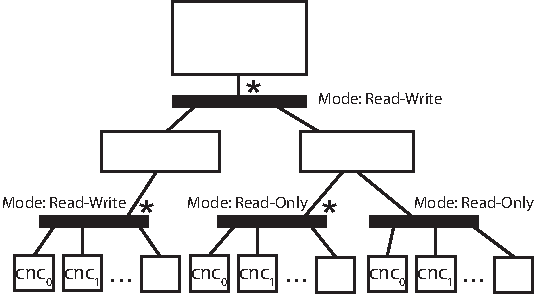
\includegraphics[scale=0.46]{figs/CNC_State.pdf}
\label{fig:depexamp:a}
}
\subfigure[{\tt distribute\_charge} depends on {\tt calc\_new\_currents}.]{ 
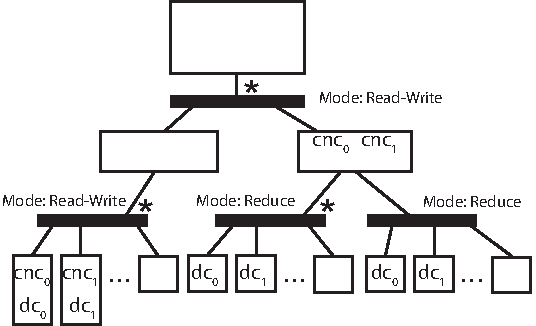
\includegraphics[scale=0.46]{figs/DC_state.pdf}
\label{fig:depexamp:b}
}
\subfigure[{\tt update\_voltages} depends on {\tt distribute\_charge}.]{
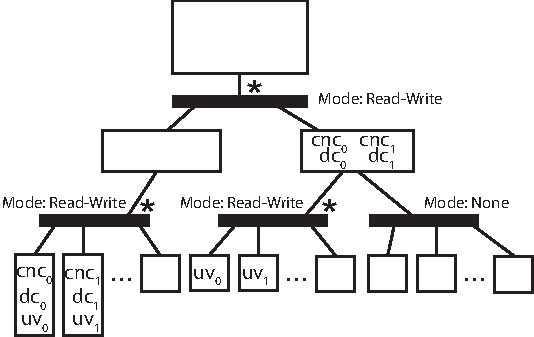
\includegraphics[scale=0.46]{figs/UV_State.pdf}
\label{fig:depexamp:c}
}
\subfigure[An {\tt update\_voltages} mapping.]{
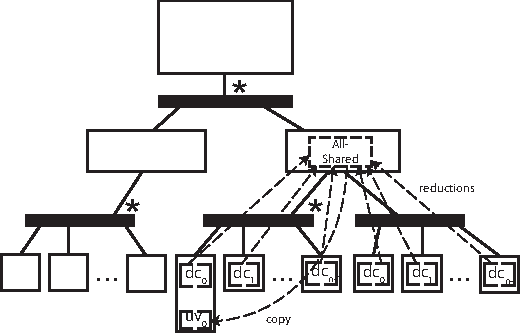
\includegraphics[scale=0.46]{figs/UV_Update.pdf}
\label{fig:depexamp:d}
}
\vspace{-2mm}
\caption{Dependence analysis examples from {\tt circuit\_simulation}. \label{fig:depexamp}}
\vspace{-6mm}
\end{figure*}

There are two parts to this analysis:
the walk from a region root to $r'$ and the off-path work
to move dependent tasks to the least common ancestor on the path.
The walk to $r'$ is bounded by the depth of the region tree.
The off-path work can be made efficient by maintaining at each node a
record of the {\em mode} of each subtree (whether the subtree has any tasks and with what privileges),
enabling the off-path search to traverse directly and only to
dependent tasks.  The off-path work is proportional to how far a task
is moved back up the region tree.  Thus, for each region argument a
task is initially placed at some depth in the forest and subsequently
only moved up towards a root, so the overall work per region is (amortized)
${\cal O}(d)$.  
%In practice, we have found this level of efficiency,
%where analyzing mapping dependences is linear in the number regions used (and not the square) and
%proportional to the depth of the region tree (and not its size)
%to be very important in minimizing the overhead of the SOOP.

We illustrate dependence analysis using the four tasks discussed
above.  Many more tasks are executed by the circuit simulation,
but this subset illustrates the important
points. Figure~\ref{fig:depexamp} shows the node region tree in three
stages.  In Figure~\ref{fig:depexamp:a}, the two tasks
{\tt calc\_new\_currents(pieces[0])} ($c_0$) and {\tt
    calc\_new\_currents(pieces[1])} ($c_1$) have been placed on their region arguments,
  which determines these two tasks are independent.
Next, in Figure~\ref{fig:depexamp:b}, the task {\tt distribute\_charge(pieces[0],dt)} ($d_0$)
has dependences with both $c_0$ and $c_1$ caused by aliasing between the pieces of the
shared node partition and the ghost node partition, so both $c_0$ and $c_1$ are moved to
the {\tt p\_nodes\_pvs[1]} region.  Finally, the task {\tt update\_voltages[1]} causes
$d_0$ to also be moved to {\tt p\_nodes\_pvs[1]} for essentially the same reason; the final
state of the node region tree is shown in Figure~\ref{fig:depexamp:c}.


\subsection{Stage 2: Distribution}
\label{sec:dist}

The first step in distribution is that $t$ waits for all tasks on which $t$ depends to
map; nothing happens to $t$ during this time.  Once $t$'s mapping
dependences are satisfied, $t$ is ready to be mapped and is placed
in the SOOP's mapping queue. At this point SOOPs on other processors may
ask to steal $t$ from its home SOOP.  The home SOOP may decline the
request, but if the request is granted, task $t$ along with a copy of
$t$'s region forest is sent to the remote SOOP.  If $t$ has not been
stolen when it reaches the head of the queue, the SOOP decides whether
to execute $t$ on the local processor or send it to another processor.
Thus, task distribution to processors in Legion is both ``pull'' (stealing) and ``push''.
The various policies (whether steal requests are granted, when to send
a task to another processor, etc.) are part of the {\em mapping interface}
and can be defined by the user (see Section~\ref{sec:mapping}).


\subsection{Stage 3: Mapping}
\label{sec:map}

%After a processor $p$ is chosen for a task, $t$ executes entirely on $p$.
%nBefore execution, however, we must {\em map} $t$, i.e., choose the
%physical instances for $t$'s logical regions.  A physical instance is assigned
%to a particular memory in the machine and holds a snapshot of the region's data
%from some point in time; a {\em valid} physical instance has data that reflects
%all the updates of all previously mapped tasks.

There are two steps to mapping a region $r$ used by
task $t$.  First, the mapper must ensure there is at least one {\em valid}
physical instance of $r$ for $t$ to use.  Not all instances have up-to-date
data at all times.  For example, if an instance of a subregion of $r$ has been written by a previous task,
it is necessary to copy that subregion back to an instance of $r$ so that $t$
sees the correct data. In the second step, the mapping interface selects one of the
valid physical instances of $r$ for $t$ to use or creates a new one.  
We focus on the first step; the mapping interface is discussed further in Section~\ref{sec:mapping}.

Each logical region in the region tree maintains a
list of its physical instances and which sibling tasks are using those
instances and with what permissions.  The important correctness
property established by stage 1 is that all
tasks on which $t$ depends map before $t$ maps and no task that depends on
$t$ maps before $t$ finishes mapping.  Thus, when $t$ maps, the region tree
will be in a state consistent with an execution in which all tasks
mapped in program order.
%Thus, the region tree when
%$t$ maps contains a consistent view of what the state of physical instances
%will be after $t$'s dependence predecessors execute.


%For example, assume there is one physical instance $s$ of
%logical region $r$ and that a task $t'$ that mapped prior to $t$ is recorded as writing a
%physical instance $s_i$ of subregion $r_i$ of $r$.  At this point there
%is no valid instance of $r$, because $s$ does not include
%the updates to $s_i$.  To restore $s$ to a valid instance of $r$ the
%system must shedule an operation after $t'$ to copy
%$s_i$ back into $s$.  


%Typical
%policies are to to choose the existing physical instance that is
%closest to $t$'s processor, or to create a new instance (by issuing a
%copy operation) in the memory closest to $t$'s processor.


Detecting or creating a valid instance of $r$ is, at its core, dependence analysis on
physical instances and thus similar to the mapping dependence analysis on logical
regions in Section~\ref{sec:dep}.  Consider mapping task $t$ with task $t'$ using
physical instance $s'$ of logical region $r'$ in the region tree.  There are four cases.
\begin{enumerate}
\item If $t'$ has only read privileges
for $r'$ it cannot invalidate any instance of $r$.

\item If $t'$ has read/write privileges for $r'$, and $r$ aliases $r'$,
   then $s'$ must be copied to an instance $s''$ of
  $\lca{r}{r'}$ and a fresh instance of $r$ created from $s''$.
%  (if either $r = \lca{r}{r'}$ or $r' = \lca{r}{r'}$ one of the two
%  copies is omitted)
Instance $s'$ is removed from the region tree.

\item If $t'$ has reduce privileges for $r'$ and $t$ has reduce
  privileges for $r$ and both use the same reduction operator, then
  nothing is done.  This is the only case in which a writer
  does not require a valid instance---because reductions can be
  reordered, combining the instances of $r$ and $r'$ (if they
  alias) can be deferred to a later consumer of the data (see case
  4).

\item If $t'$ has reduce privilege for $r'$ and $t$ has read, write, 
  or reduce privileges with a different operator than $t'$
  for $r$, and $r$ aliases $r'$, then $s'$ must be
  reduced (using $t'$'s reduction operator) to an instance $s''$ of
  $\lca{r}{r'}$ and then a fresh instance of $r$ created from $s''$.
%  (If $r' = \lca{r}{r'}$ the reduction is unneeded, and if $r =
%  \lca{r}{r'}$ the copy is unneeded.) 
Instance $s'$ is removed from the region
  tree.
\end{enumerate}

%Not all of these cases can occur simultaneously for a particular
%region argument $r$ of task $t$.  There may always be multiple
%previous readers (case 1), but the mapping dependence analysis
%guarantees that there would only be one previous writer (case 3) or
%one or more reducers (cases 2 and 4).  
To map $r$, we walk from $r$'s
root ancestor in the region forest to $r$, along the way exploring
off-path subtrees to find region instances satisfying cases 2 and
4. The details and analysis are similar to the implementation of dependence
analysis in Section~\ref{sec:dep}; the amortized work per region mapped
is proportional to the depth of the region forest and independent of
the number of tasks or physical instances.

As part of the walk any required copy and reduction operations are
issued to construct a valid instance of $r$.  These operations are
deferred, waiting to execute on the tasks that produce the data they
copy or reduce. Similarly, the start of $t$'s execution is made
dependent on completion of the copies/reductions that construct the
instance of $r$ it will use.

Figure~\ref{fig:depexamp:d} shows part of the mapping of task {\tt update\_voltages[0]}; we focus
only on the shared nodes.
Because the immediately preceding {\tt distribute\_charges} tasks all performed the same reduction
on the shared and ghost nodes they were allowed to run in parallel.  But {\tt update\_voltages[0]}
needs read/write privilege for {\tt pieces[0].rn\_shr}, which forces all of the reductions to be merged
back to an instance of the {\tt all-shared} nodes region, from which a new instance of {\tt pieces[0].rn\_shr} is copied and used by {\tt update\_voltages[0]}.

%
% FIXME   CUT
%
%Figure~\ref{fig:gpumapping} shows a timeline of our mapping of the
%circuit simulation on a cluster of GPUs.  The $i$th private node and
%wire regions are mapped to the $i$th GPU's DRAM and simply left there
%for all three phases of the simulation.  The $i$th shared and ghost
%regions are mapped to zero-copy memory most of the time, but, as just
%illustrated, must be reduced out to the all-shared node region in the
%global memory (which is managed by GASNet) and then a new instance of the shared
%subregions created with the updated information before the {\tt
%  update\_voltages} tasks execute.  A similar situation arises before
%{\tt calc\_new\_currents} tasks run again: the updates to the shared
%nodes by {\tt update\_voltage} must be propagated to the ghost nodes
%before continuing.
%
%\begin{figure}
%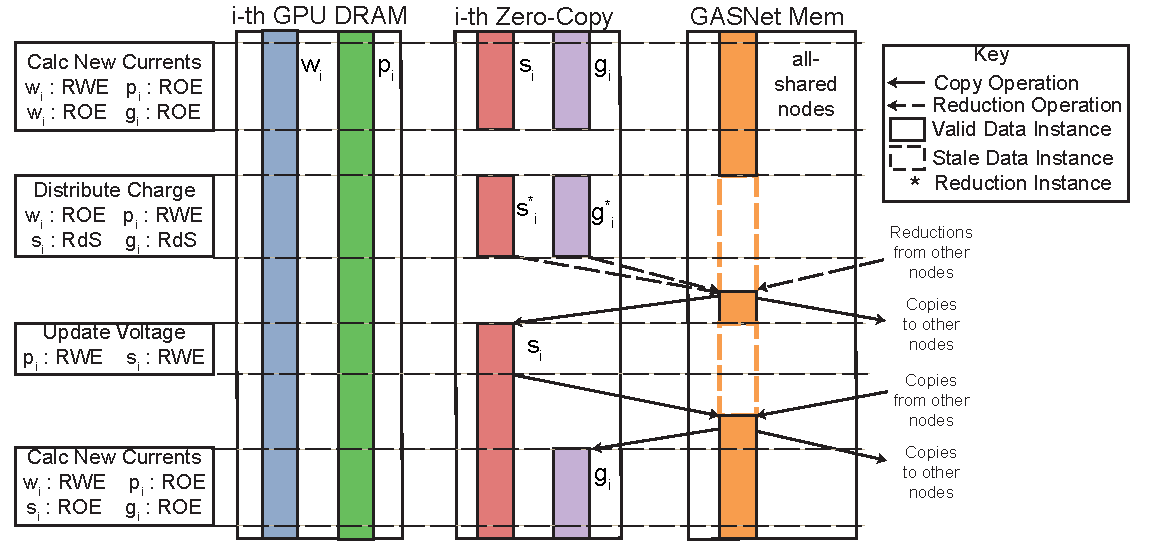
\includegraphics[scale=0.48]{figs/CircuitMem.pdf}
%\caption{Tasks and data for the circuit simulation on a cluster of GPUs.}
%\label{fig:gpumapping}
%\end{figure}

\subsection{Stage 4: Execution}
\label{sec:exec}

After a task $t$ has been mapped it enters the execution stage of the SOOP.  When all of
the operations (other tasks and copies) on which $t$ depends have completed, $t$ is
launched on the processor it was mapped to.  When $t$ spawns subtasks, 
they are registered by the SOOP on which $t$ is executing, using $t$ as the parent task 
and $t$'s region arguments as the roots of the region forest.  Each child of $t$ traverses
the SOOP pipeline on the same processor as $t$, possibly being mapped to a 
SOOP instance on a different processor to execute.   


\subsection{Stage 5: Clean-Up}
\label{sec:clean}

Once task $t$ is done executing its state is reclaimed. Dependence
and mapping information is removed from the region tree.  The most involved aspect of
clean-up is collecting physical instances that are no longer in use,
for which we use a distributed reference counting scheme.



\section{Mapping}
\label{sec:mapping}

While the Legion programming model describes locality and independence information abstractly,
to run a Legion application on a machine we must make concrete decisions about
where tasks will be run and where region instances will be placed.  Instead of placing
the burden of decision making on the programming system, we introduce a programmable mapping
interface that gives a programmer total control over how these decisions are made.  Armed
with this interface, the programmer can then specify application- or machine-specific
mapping decisions that would be difficult for a general-purpose programming system to infer.
In this section we describe the general mapping interface (Section \ref{sec:mapinterface}),
our base implmentation of this interface (Section \ref{sec:defmapper}), and the benefits
of creating custom mappers (Section \ref{sec:custommap}).

\subsection{Mapping Interface}
\label{sec:mapinterface}
A mapper is any object that implements the mapping interface.  The mapping interface
consists of ten function calls that the runtime will make to request direction from
the programmer about how a program should be executed.  To aid in performing the 
decisions made in these calls the mapper has access to a simple 
interface for inspecting the properties of the machine on which it is running.  This includes 
information about all the processors and their kinds (i.e. CPU,GPU), as well as the memories visible
to each processor and their latencies and bandwidths.  For brevity we only
discuss three of the mapping interface calls.

\begin{itemize}
\item {\tt select\_initial\_processor} - for each task the runtime system will
ask the mapper to which processor the task should be sent.  The mapper 
can choose to keep the task on the local processor or send it to any other processor
in the system.

\item {\tt permit\_task\_steal} - when handling a steal request from another processor
the runtime will ask the mapper to decide which tasks are allowed to be stolen.  
By always returning an empty set, the mapper can disable stealing.

\item {\tt map\_task\_region} - for each logical region requested for a task, the
runtime will query the mapper for a prioritized list of memories where a physical instance for this
task should be placed.  To aid the mapping decision the runtime provides a list of the current valid physical intances
of the logical region.  The mapper returns a list of memories in which the runtime
should attempt to either reuse or manifest a physical instance of the logical region.  The
runtime traverses this list and searches for a currently valid instance.  If none can be
found, it attempts to allocate a physical instance and then issue the necessary copies
to retrive the valid data.  If both options fail, it moves on to the next memory in the list.
\end{itemize}

There are two very elegant properties of this mapping interface.  The first property is
that all decisions made by a mapper are orthogonal to the correctness of the program and can only 
impact performance.  Regardless of where a mapper chooses to place a task or map a region, 
the runtime will always schedule tasks and copies in accordance with the privileges and 
coherence properties specified in the Legion program.  Therefore when writing an application
in Legion, a programmer can begin by using the default mapper and later optimize his program
by creating a custom mapper and gradually refining its mapping decisions.

The second useful property of the mapping interface is that it isolates machine-specific decisions
to a specific module of code.  As a result, Legion programs are highly
portable.  To port a Legion program to a new architecture, a programmer only has to
implement a new mapper with decisions specific to the new architecture. 

\subsection{Default Mapper}
\label{sec:defmapper}
To make writing Legion applications easier, we provide a default mapper implementation that
can be used to get an application working quickly at a moderate performance level.  The 
default mapper employs a simple scheme for mapping tasks and regions.  When
{\tt select\_initial\_processor} is invoked for the default mapper, it first checks for which kind of processors
the task has variants (i.e. GPU).  If the fastest variant is for the kind of processor the mapper is managing
it will choose to keep the task local, otherwise it will send the task to the closest processor of the
fastest variant kind.

The default mapper employs a Cilk-like algorithm for task stealing\cite{CILK95}.  Tasks are kept local
to their target processor whenever possible and only moved when stolen.  Unlike Cilk, the default mapper
has the information necessary for locality-aware stealing.  When {\tt permit\_task\_steal} is called for a task, 
the default mapper inspects the logical regions for the task being stolen, and will mark that other tasks using 
the same logical regions should be stolen as well.

For calls to {\tt map\_task\_region}, the default mapper constructs a stack of memories ordered from best-to-worst
by bandwidth from the local processor.  This stack is then returned as the location of memories to be used for
mapping each region.  Note that this is a greedy algorithm that works well for the common case, but can cause some 
regions to be pulled unnecessarily close to the processor and consume precious fast memory space.  

\subsection{Custom Mappers}
\label{sec:custommap}
To optimize a Legion program or library, programmers can create one or more custom mappers.  
For each Legion task call the programmer specifies which mapper should be invoked by the runtime for
mapping that particular task.  This allows for the composition of Legion applications and libraries
each with their own custom mappers.

Each custom mapper extends the default mapper.  A programmer only has to override the functions necessary 
for creating a custom mapping.  Custom mappers can be used to create totally static mappings, 
mappings that memoize their results, or even totally dynamic mappings.  We describe examples of 
custom mappers in Section \ref{sec:exp}.





\section{Experiments}
\label{sec:exp}



\begin{figure}
{\footnotesize
\begin{tabular*}{3.5in}{l|ccc}
Cluster & Sapling & Viz & Keeneland \\
\midrule
Nodes   &   4     &  10 &  32 (120) \\
CPUs/Node & 2x Xeon 5680 & 2x Xeon 5680 & 2x Xeon 5660 \\
HyperThreading & on & off & off \\
GPUs/Node & 2x Tesla C2070 & 5x Quadro Q5000 & 3x Tesla M2090 \\
DRAM/Node & 48 GB & 24 GB & 24 GB \\
Infiniband & 2x QDR & QDR & 2x QDR \\
\end{tabular*}
}
\vspace{-2mm}
\caption{System configurations used for the experiments. \label{fig:systems}}
\vspace{-6mm}
\end{figure}

% FIXME
% This is a nice paragraph, but it doesn't belong here; perhaps in the mapping section
% if we have space.
%
%Nodes with multiple instances of different resources are challenging
%for existing programming models with flat system views (e.g., MPI).
%They must either lump resources together and ignore internal irregularities (e.g. NUMA
%in multi-socket x86 systems), or divide a single physical node into
%multiple smaller nodes, ignoring the better affinity between sockets/GPUs/etc.
%on the same node. In contrast, the machine model used by Legion is based on an
%affinity graph of CPUs and GPUs and accurately captures complex
%machine hierarchies.
%
% FIXME
%   I cut this from the above, commented-out paragraph because it was a digression. 
%  
% and either wasting or over-subscribing some resources when
%the quantities of different resources don't share a common divisor.


We evaluate the efficiency and scalability of Legion using
three applications on three clusters (see Figure~\ref{fig:systems}).  All three
clusters were Linux-based, and the Legion runtime was built using pthreads for
managing CPU threads, CUDA\cite{CUDA} for GPUs, and GASNet\cite{GASNET07} for
inter-node communication.  The RDMA features of GASNet were used to create a 
globally addressable, but relatively slow, {\em GASNet memory} that is accessible
by all nodes.
For each application, multiple problem sizes were used, and each size problem was
run on subsets of each machine ranging from the smallest (a single CPU core or GPU)
to the largest or near-largest (except Keeneland, where we limited
runs to 32 nodes to get sufficient cluster time).
By examining performance of the same size problem over progressively larger
machines, we measure Legion's strong scaling.
By increasing the problem size as well, we also measure weak scaling.

\subsection{Circuit Simulation}
\label{subsec:exp_ckt}

The first experiment we investigate is the distributed circuit simulation described in 
Section~\ref{sec:ex}.  The Legion SOOP runtime handles all of the resource allocation, 
scheduling, and data movement across the cluster of GPUs.  In particular,  
Legion's ability to efficiently move the irregularly partitioned
shared data around the system while keeping the private nodes and wires resident in
each GPU's framebuffer memory is critical to achieving good scalability.

Circuits of two different sizes were simulated.  The first had 480K wires, connecting
120K nodes.  The second is twice as large, with nearly 1M wires connecting 
250K nodes.  In addition to running these tests on varying numbers of
nodes, the number of GPUs used by the runtime was also varied.  In no case did the 
changes to nodes or number of GPUs per node require changes to the application code.

The circuit simulation has a simple application-specific mapper.  At initialization
time, the mapper queries the list of GPUs in the machine and identifies each GPU's
framebuffer memory and {\em zero-copy} memory (pinned memory that both the GPU and
CPUs in the system can access directly).  Once the circuit is partitioned, the partitions
are assigned a home GPU in round-robin fashion.  Every task related to that partition is
then sent to the home GPU, with no task stealing allowed.  
(In a well-partitioned circuit,
load imbalance is low enough that the cost of moving the private data for a piece from one
GPU to another outweighs any benefits.)

  The regions for the tasks are mapped as 
shown in Figure~\ref{fig:gpumapping}.  Wires and private node data are kept in each GPU's
framebuffer at all times.  An instance of the ``all-shared nodes'' region is placed in
GASNet memory and instances for just the shared and ghost nodes needed by each GPU
are placed into that GPU's zero-copy memory.  This enables the application kernels
to access the data as well as the necessary inter-node exchanges of data via the GASNet
memory.

\begin{figure}
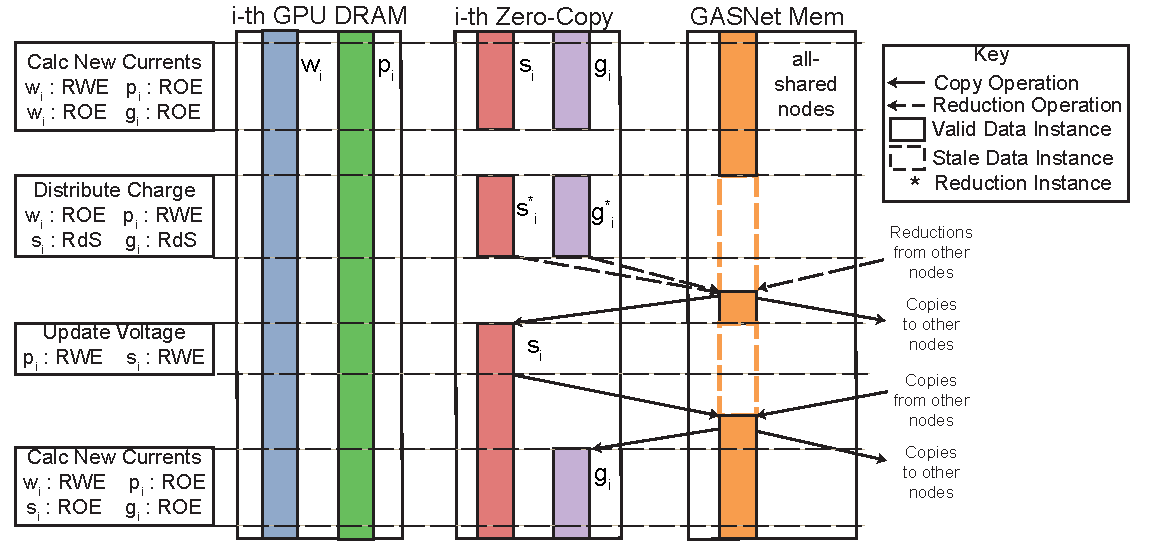
\includegraphics[scale=0.48]{figs/CircuitMem.pdf}
\caption{Tasks and data for the circuit simulation on a cluster of GPUs.}
\label{fig:gpumapping}
\end{figure}

Figure~\ref{fig:ckt_speed} shows the performance of the Legion circuit simulation relative
to a hand-coded single-GPU implementation written in CUDA.  The hand-coded implementation is
able to keep the entire simulation state in fast framebuffer memory.  Each line shows the scaling of
a particular problem size as the number of nodes is varied.  Our results demonstrate
excellent strong scaling, with speedups of 39.0X for the small problem on 48 GPUs and 
62.5X for the larger problem size on 96 GPUs.  The inset in the graph shows the relative
performance for small numbers of GPUs.  On a single GPU, our Legion implementation
is within 5\% of the performance of the hand-coded simulation.

Figure~\ref{fig:ckt_overhead} shows the fraction of the overall simulation time (summed over
all nodes) spent in the application kernels compared to the various pieces of the Legion
SOOP runtime.  As the node count increases, the non-communication overhead stays relatively constant.
As expected the communication overhead grow linearly with number of nodes.

\begin{figure}
\subfigure[Circuit simulation speed relative to single-GPU implementation.]
{
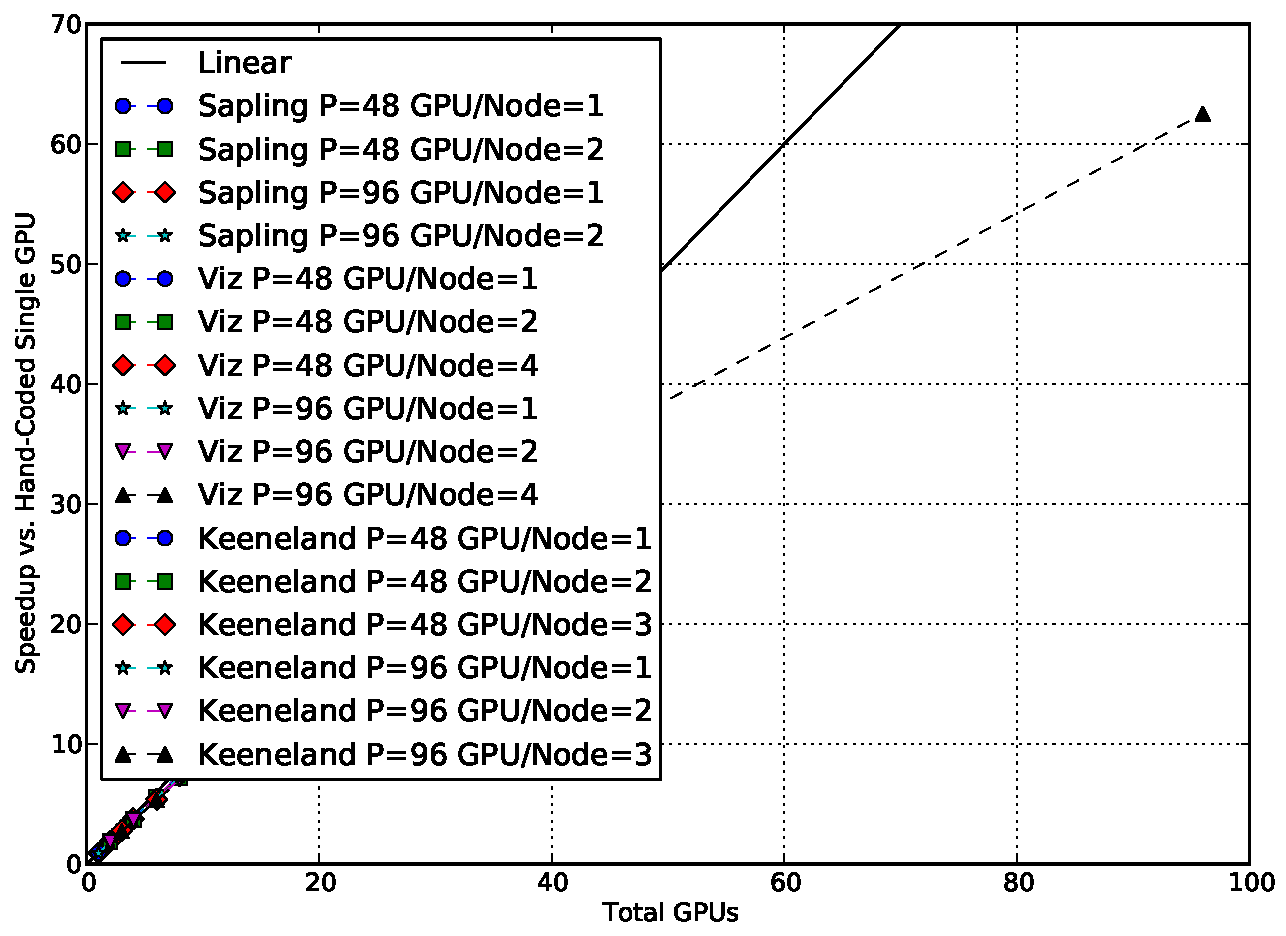
\includegraphics[scale=0.4]{figs/circuit_speedups.pdf}
\makebox[0pt][r]{
\raisebox{0.25 in}{
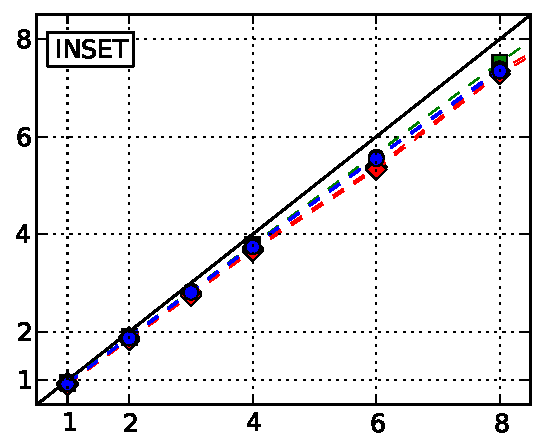
\includegraphics[scale=0.4]{figs/circuit_speedups_zoom.pdf}
}
}
\label{fig:ckt_speed}
}

\subfigure[Overhead of circuit simulation on Keeneland with 3 GPUs/node.]
{
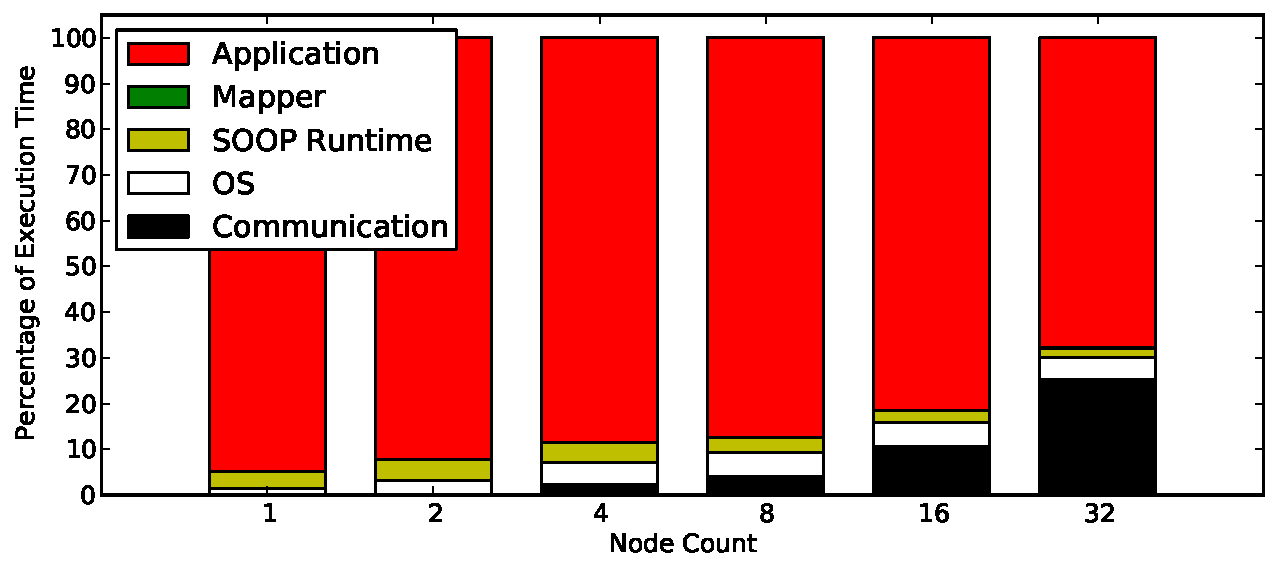
\includegraphics[scale=0.4]{figs/circuit_overhead.pdf}
\label{fig:ckt_overhead}
}
\vspace{-2mm}
\caption{Circuit simulation results.}
\vspace{-6mm}
\end{figure}

\subsection{Particle Simulation}
\label{subsec:exp_fluid}

Our second experiment is a port of the \emph{fluidanimate} benchmark
from the PARSEC benchmark suite\cite{bienia11benchmarking}, which does a
particle-based simulation of an incompressible fluid.  Each particle
interacts only with other nearby particles. The benchmark divides the
space in which the fluid can move into a three-dimensional array of
cells such that the range of interaction is limited to just the cells
adjacent (including diagonals) to the one a particle resides in.  The
application divides the array into {\em grids} and assigns each grid to
a thread.  Per-cell locking safely accesses particles in
cells that lie on the edge of a grid.  This fine-grained locking
scheme along with the assumption of a shared address space gives
good scaling in a multi-core processor, but rules out any attempt to run
beyond a single node.

To extend the scaling further, our port uses region partitioning to
divide the array into grids in a similar way, but avoids relying
on shared memory to handle interactions between grids.
Instead, the Legion version creates
explicit ghost copies of cells on grid boundaries and uses
those ghost cells to exchange information between the grids.

The particle simulation's mapper is very simple: it maps one grid's
tasks onto each processor and maps all that grid's regions (both
internal and ghost regions) into that processor's system memory.  The
exchange of ghost cell data between processors is handled by the
Legion runtime as a ghost cell region is alternately mapped to two
different memories.

Figure~\ref{fig:fluid_single} compares the performance of the Legion
implementation against the PARSEC version, using a relatively small
problem (300K particles on a 15x21x15 array of cells).  Speedups for
both the Legion and threaded PARSEC implementations are measured 
relative to PARSEC's serial version, which eliminates all locking
operations.  Between 1 and
4 threads, the PARSEC and Legion results are nearly indistinguishable,
indicating neither the Legion runtime nor the restructuring of the
implementation to allow multi-node scaling impose any significant
overhead.
%It's possible that the use of explicit ghost cells rather than fine-grained sharing of cache lines might be a net win.  
At 8 threads and above, performance begins to vary.  Both the Legion
and PARSEC versions on Viz flatten out as they over-subscribe the 12
physical cores.  On Sapling, which has HyperThreading enabled,
deviations from linear begin sooner as the operating system's
thread placement choices begin to matter.

To measure scaling beyond a single node, three different problem sizes
were run for each of the three systems (Figure~\ref{fig:fluid_multi}).
For the smallest problem (300K particles), we observe a 20\% speedup
from 1 to 2 nodes (16 threads total), but slow
down beyond that due to communication overhead---at 4 nodes there are
twice as many ghost cells as interior grid cells.  The larger problem
sizes (2.4M and 19M particles) do much better, with scaling of up to
5.4x when going from 1 node up to 16 because of a lower
communication-to-computation ratio.

%Although the particle simulation being performed is on a regular array of cells, it turns out that the
%distribution of particles amongst the cells is very irregular.  The simulation models gravity, which points in
%the -Y direction, so the particles are clustered mostly in the lower half of the cell array.  The PARSEC
%implementation works around this imbalance by only slicing the cell array through the X and Z axes, yielding
%grids that are uniformly populated, even if the number of boundary cells (for which locks must be used) is
%increased above the minimum. MORE TEXT NEEDED HERE

\begin{figure}
\subfigure[Single-node particle simulation speed.]
{
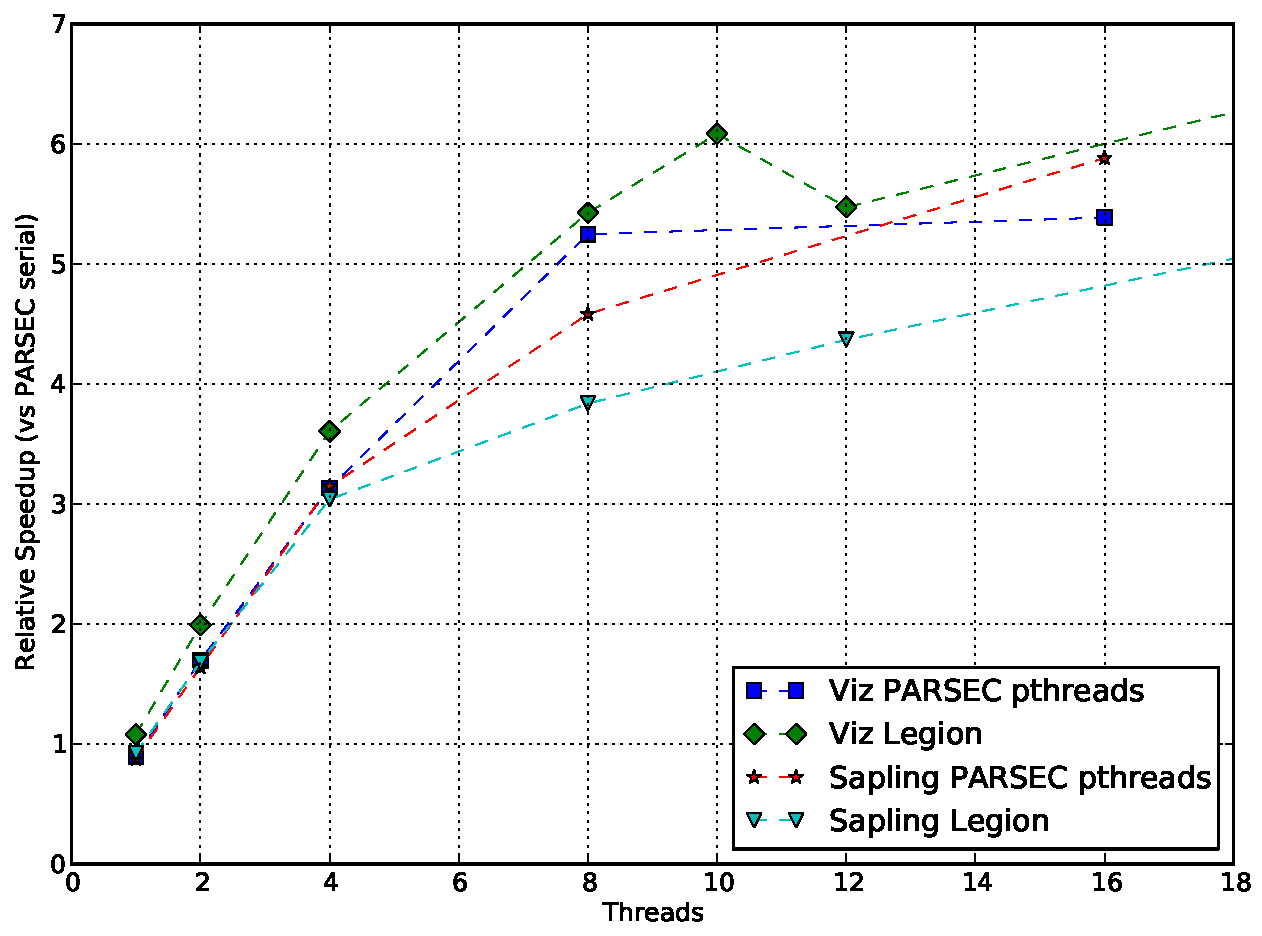
\includegraphics[scale=0.4]{figs/fluid_singlenode.pdf}
\label{fig:fluid_single}
}

\subfigure[Multi-node scaling.]
{
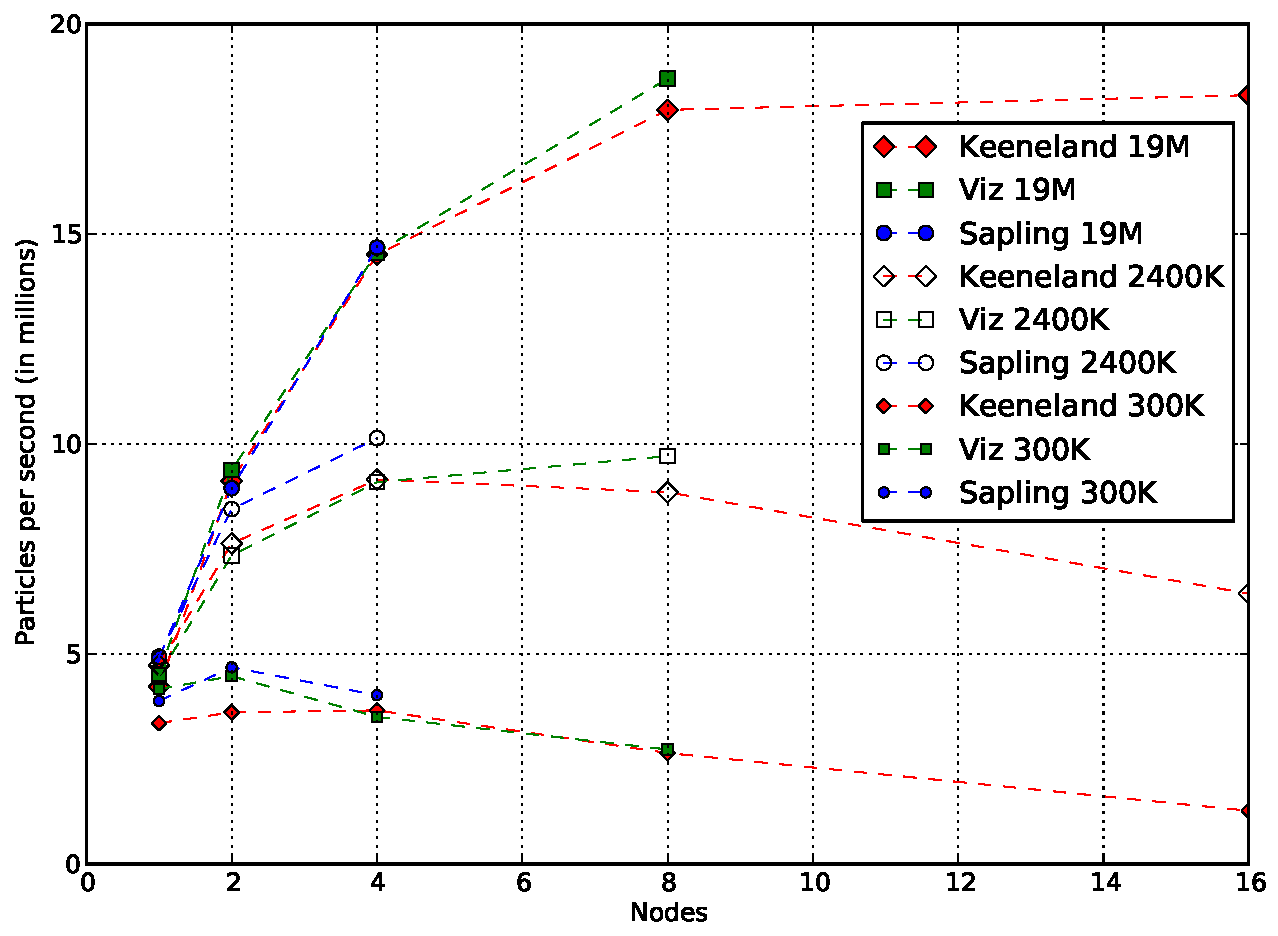
\includegraphics[scale=0.4]{figs/fluid_multinode.pdf}
\label{fig:fluid_multi}
}

%\subfigure[Effect of load-balanced partitioning.]
%{
%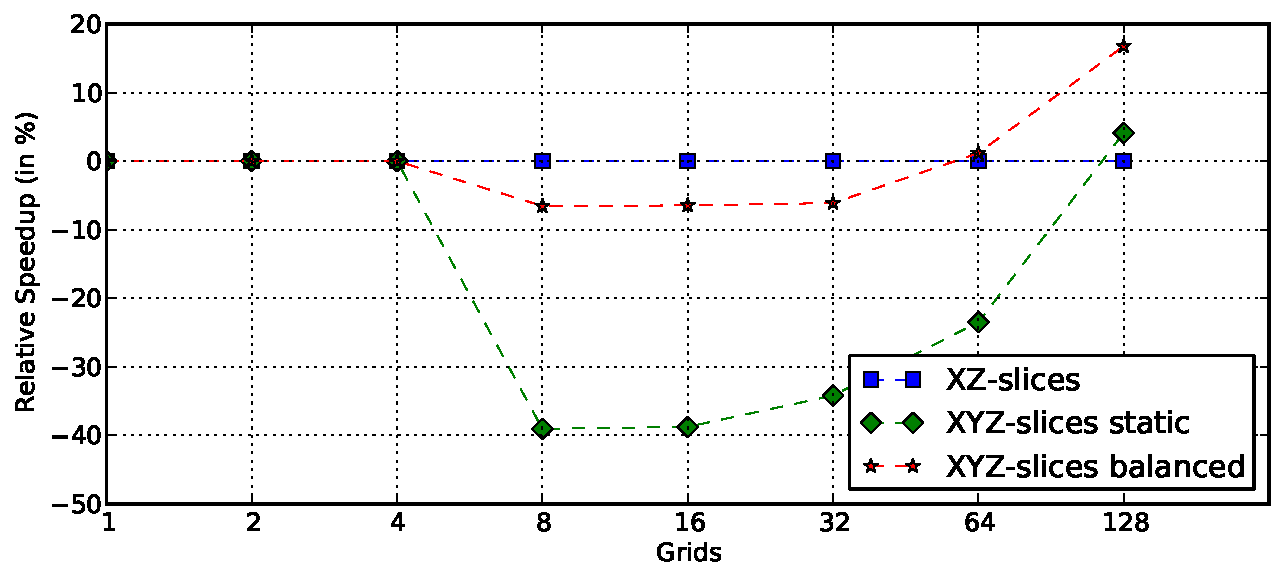
\includegraphics[scale=0.4]{figs/fluid_balance.pdf}
%\label{fig:fluid_balance}
%}
\vspace{-2mm}
\caption{Fluid simulation results.}
\vspace{-6mm}
\end{figure}

\subsection{Adaptive Mesh Refinement}
\label{subsec:exp_amr}
Our final application is based on the third heat equation example from
the Berkeley Labs BoxLib project \cite{BoxLib}.  This application is a
three-level adaptive-mesh-refinement (AMR) code that computes a first
order stencil on a 2D mesh of cells.  
%The simulation iterates for many time steps.  
Updating the simulation for one time step consists of
three phases.  In the first phase, the boundary cells around a box at
a refined level linearly interpolate their values from the nearby
cells at the next coarsest level.  The second phase performs the
stencil computation on each cell in every level.  In the third phase,
cells at a coarser level that have been refined are restricted to the
average of the cells that they physically contain at the next finest
level of refinement.

Achieving high-performance on this application is particularly
challenging for several reasons.  First, the application has a very
high communication-to-computation ratio which, for a fixed problem
size, begins as being memory bound and with increasing node count
becomes network bound as the perimeter-to-area ratio of cell grids
increases.  Second, when choosing how to partition cells into grids,
the programmer must consider the locality between cells within a
level as well as across levels.  For
cross-level cell dependences, mapping decisions must be made at
runtime as the location of refinements are dynamically determined.
Finally, this application has parallelism both
between tasks running at the same level and tasks running across
levels, leading to complicated input-dependent data dependences.

BoxLib's implementation partitions cells within a level 
into a number of grids based on the number of nodes in the
machine and distributes one grid from each level to each node.  This
optimizes for memory bandwidth and load balance, but does not 
exploit cross-level locality between grids from
different levels of refinement.  Furthermore, BoxLib does not block
grids into sub-grids to take advantage of intra-grid locality.

Our Legion implementation performs two optimizations that allow us to
outperform BoxLib.  First, for each level of
refinement we recursively partition the logical region of cells based
on the number of nodes in the machine and the sizes of the L2 and L3 caches.
%Legion allows us to describe locality for many levels of
%the memory hierarchy instead of just at the node-level.
Our second optimization takes advantage of the cross-level locality.
We wrote an application-specific mapper that dynamically discovers
relationships between grids at different levels of refinement.  The
mapper dynamically performs intersection tests between logical regions
containing grids of different refinement levels.  If the mapper
discovers overlaps between grids from different levels, the mapper
places them on the same node in the machine.  The
mapper memoizes the intersection tests to amortize their cost.  The
mapper also dynamically load balances by distributing unconstrained
grids from the coarsest level onto under-loaded nodes.

We compared our Legion implementation against BoxLib on three
different problem sizes with a fixed number of cells per level of
refinement, but with randomly chosen refinement locations.  BoxLib
also supports OpenMP and we took their best performance from using 1,
2, 4, or 8 threads per node.  Our Legion implementation always uses
one thread per node to illustrate that in this application locality is
significantly more important than parallelism.  

Figure~\ref{fig:amr_total} gives the results.
On just one node, blocking for caches using Legion achieves up to 2.6X
speedup over BoxLib.  As node count increases, the mapper's
ability to exploit cross-level locality further increases
the performance advantage to 5.4X by reducing the total
communication costs.

As the node count increases the AMR code becomes highly dependent on
interconnect performance.  BoxLib performs much better on Keeneland
than on Viz due to the better interconnect.  
At higher node counts BoxLib
begins to catch up (see Figure~\ref{fig:amr_keeneland})
because our intra-level ghost-cell exchange 
uses GASNet memory to exchange ghost cells, requiring a
linear increase in network traffic with the number of nodes.  BoxLib
uses direct node-to-node exchanges of ghost cells, similar to
our fluid application.  A future implementation of our AMR code will
employ a similar ghost cell exchange algorithm to improve scalability.

\begin{figure}
\subfigure[Sapling results.]
{
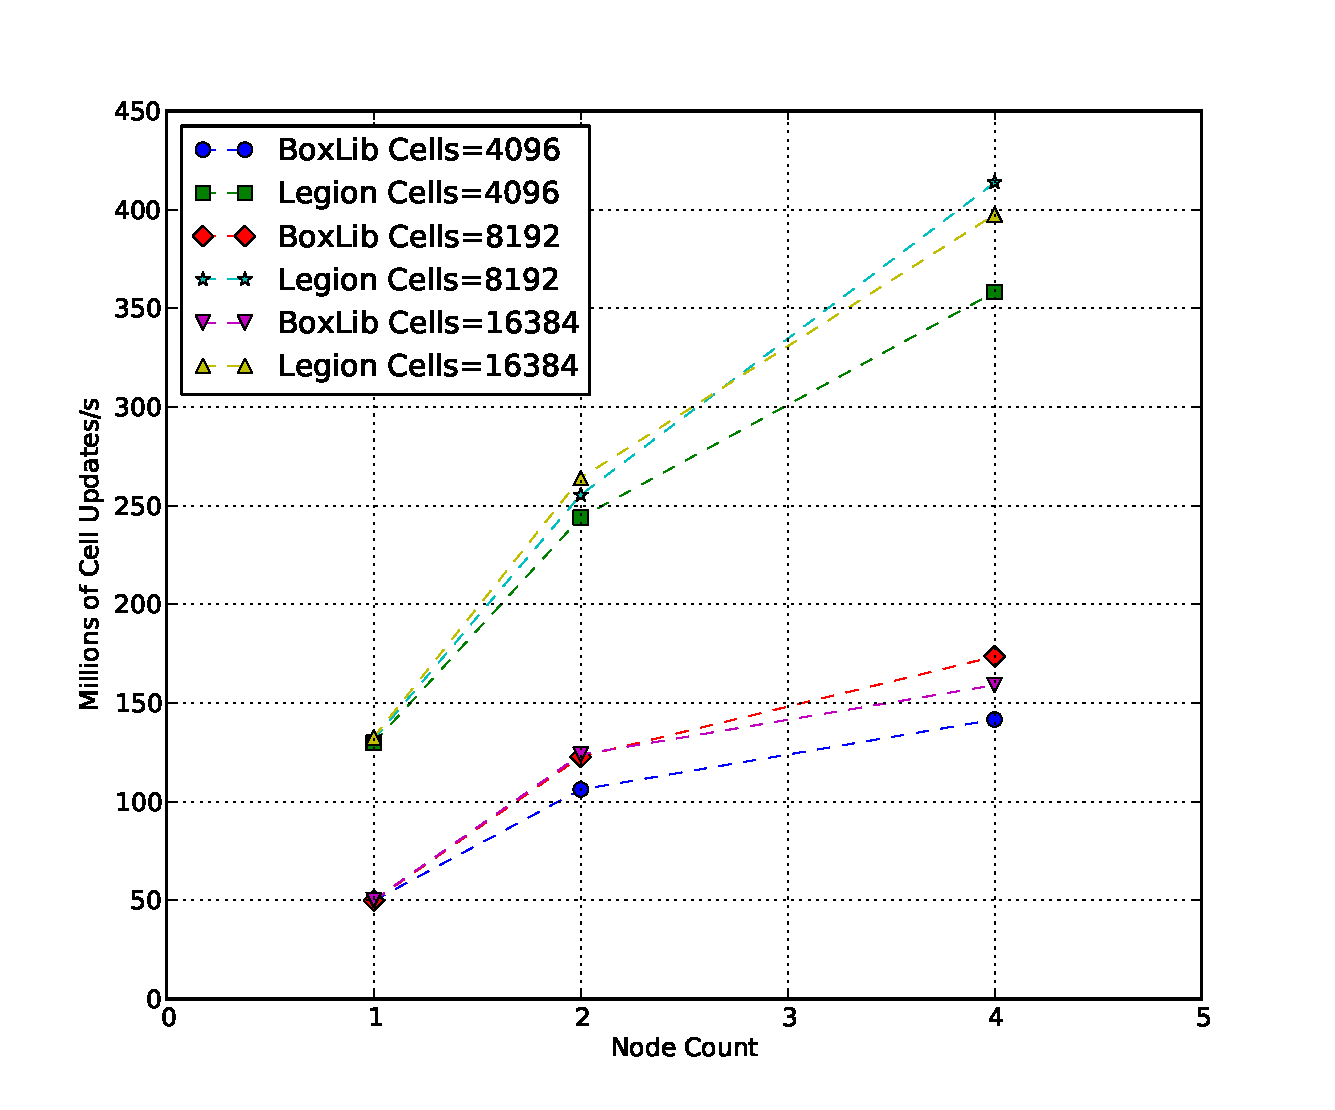
\includegraphics[scale=0.4]{figs/Sapling_amr.pdf}
\label{fig:amr_sapling}
}

\subfigure[Viz results.]
{
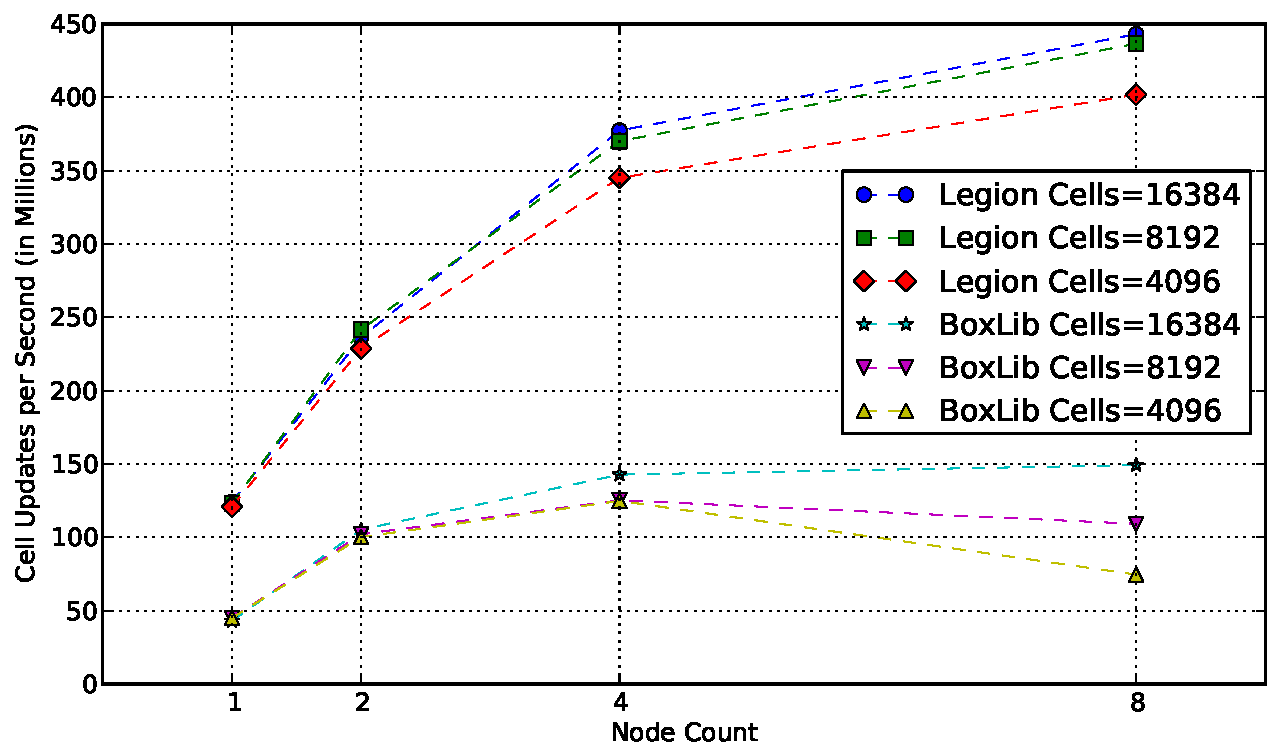
\includegraphics[scale=0.4]{figs/Viz_amr.pdf}
\label{fig:amr_viz}
}

\subfigure[Keeneland results.]
{
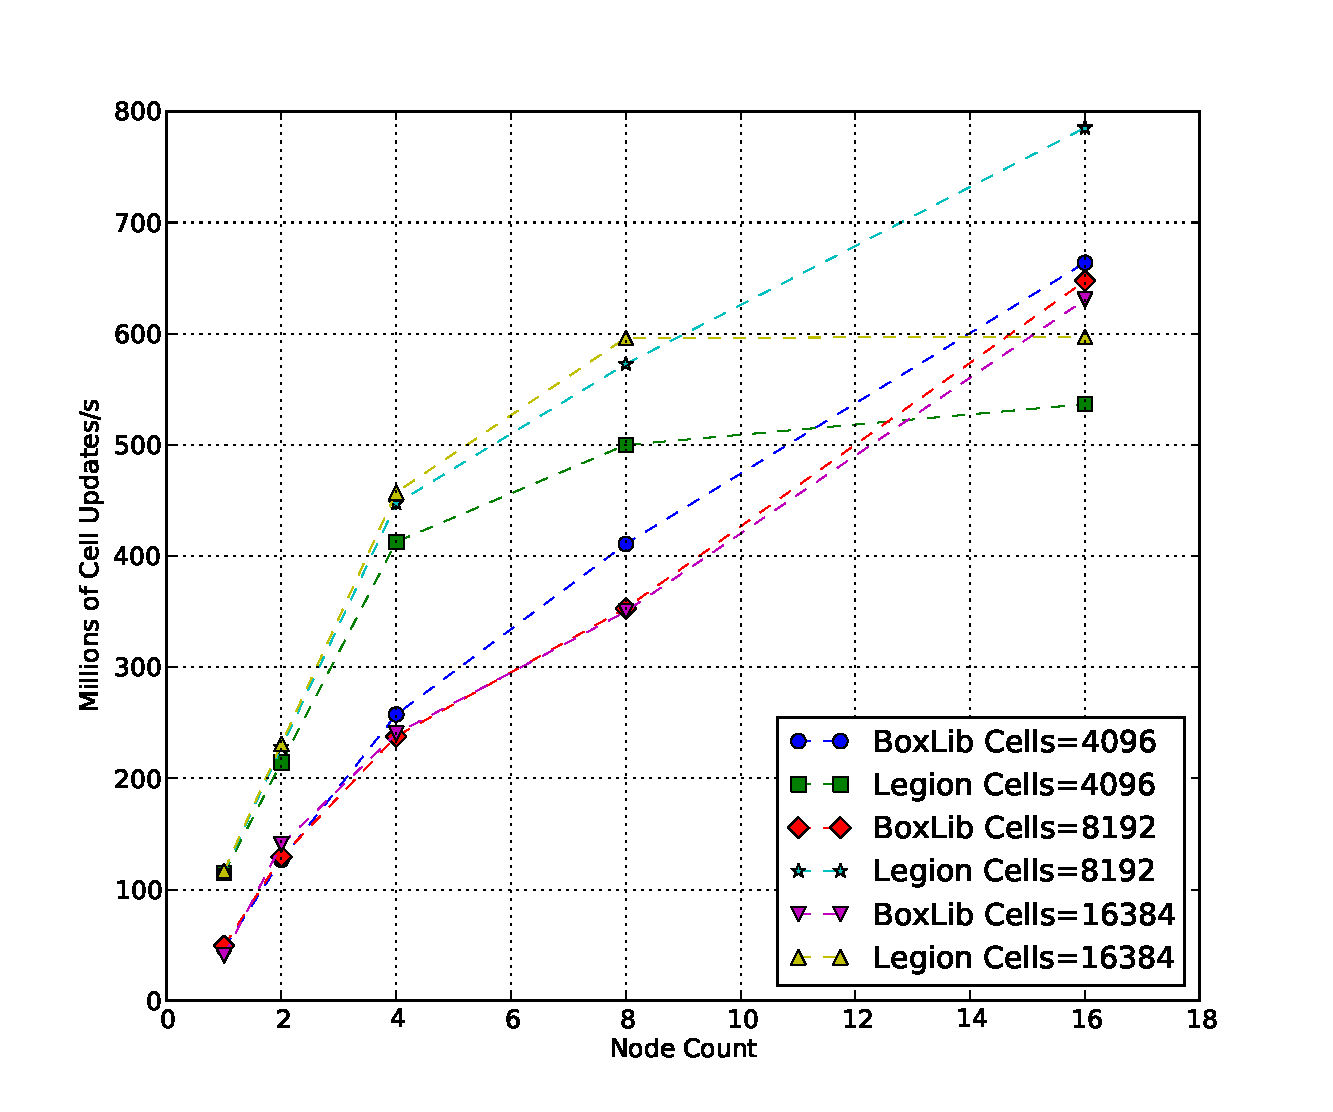
\includegraphics[scale=0.4]{figs/Keeneland_amr.pdf}
\label{fig:amr_keeneland}
}
\vspace{-2mm}
\caption{Throughput of adaptive mesh refinement code. \label{fig:amr_total}}
\vspace{-6mm}
\end{figure}


\section{Related Work}
\label{sec:related}
Legion is most directly related to Sequoia \cite{Fatahalian06}.  Sequoia is array-based, with
a limited repetoire of ways to partition arrays.  Sequoia is a static language with a single unified hierarchy
of tasks and data; Legion is more dynamic with separate task and region hierarchies.

Deterministic Parallel Java (DPJ) is the only other region-based parallel system of which we are
aware\cite{Bocchino09}.  While there are similarities in the permission system and we have
reused some DPJ notation, there are differences stemming from DPJ's static approach.
Regions in Legion are first-class and can be created, partitioned, packed, and unpacked 
dynamically, allowing programmers to compute data organization at runtime; like Sequoia, DPJ
partition schemes must be statically decided.  Legion allows 
programmers to create multiple partitions of the same region to give different 
views onto the same data, which is not possible in DPJ.  
%DPJ only supports the 
%equivalent to Legion's exclusive and atomic coherence modes \cite{Bocchino11} 
%while Legion provides safe execution even in simultaneous environments.  
There is also a difference in emphasis: DPJ requires shared memory, while Legion 
is designed for distributed heterogenous machines.

Chapel \cite{Chamberlain:Chapel} and X10 \cite{X1005} also provide some Legion-like facilities.
Chapel's domains and X10's places provide the programmer with a 
mechanism for expressing locality, similar to regions in Legion.  However, domains
and places are not used for independence analysis to discover parallelism.
In contrast, Jade uses annotations to describe
data disjointness,  and like Legion leverages the disjointness information
to discover parallelism, but lacks a region system to name and organize unbounded collections of objects \cite{Rinard98}.  

% Unclear to me what subtleties need to be pointed out here and explained
% to properly differentiate our work
Many efforts use static region systems for  memory management (e.g., \cite{Tofte94, Grossman02}).
Our system is more closely affiliated with dynamic region systems used for expressing locality for performance \cite{Gay01}.

%In addition to region languages with static type systems, there have been several
%dynamic region languages.  Cyclone uses both a static type system and dynamic
%region checks to enforce memory safety properties of C programs\cite{Grossman02}.
%Gay and Aiken introduced RC which reference counts regions dynamically and uses
%a static type system to reason about effeciently garbage collecting regions\cite{Gay01}.

There have been many type and effect systems for ownership types
\cite{Boyapati03} including ones that leverage nested regions for describing
relationships \cite{Clarke02,Cameron07}.  However, ownership type and effect systems
are primarily used for reasoning about determinism in object oriented languages and
don't capture the range of disjointness properties that can be specified in Legion.

Reasoning about disjoint heap data is the strong suit of separation logic \cite{Reynolds02}.  
Concurrent separation logic\cite{Brookes04} has been 
used both to parallelize sequential programs\cite{Raza09,Gotsman07} and to provide 
a mechanism for reasoning about independence\cite{Hayman06}.
While we have borrowed some separation logic notation, we ultimately chose to use a 
permissions system as our primary formalism because separation logic does not easily
support reasoning about the interleaving of operations to non-disjoint regions of memory.

% I'm also not sure how much detail to go into here.  DPJ spends a lot of time
% on these papers, but I'm not sure I understand all the details of these papers.
% DPJ also cites Lu06 here, but I'm not sure if we have to
%Type and effect systems have also been used to reason about regions.  FX presented
%the original type and effect system on regions \cite{Lucassen88}, but was restricted 
%to using a finite number of regions and was incapable of describing nested data
%structures.  

% Do we need to enumerate what these disjointness properties are (DPJ does)
%Type and effect systems have also been used in the context of parallelism to discover
%deadlocks and race conditions \cite{Boyapati02,Abadi06,Jacobs08}, but do not present 
%any mechanism for discovering parallelism.

%Still not sure what we want to put here.
% DPJ sites additional separation logic papers but they didn't seem very similar.
% Let me know if you think we should include them as well.



%
\section{Conclusion}
We have presented Legion, a programming model and
type system for expressing locality and independence
to target heterogeneous, distributed parallel architectures.  
We implemented both a portable high-level and machine 
abstraction low-level runtime to support the Legion 
programming model.  Our implementation of Legion demonstrated
speedups up to 5.9X on a cluster of GPUs.



\bibstyle{IEEEtran}
\bibliography{bibliography}

\end{document}


